\section{Jet ranking for signal models\label{app:jetRanking}}

As discussed in Section~\ref{sec:susy}, when setting limits only 4 out of 9 jet categories (but all \nb/\scalht bins
within each category) are considered to extract the final result. 
To choose the 4 jet multiplicity categories that are combined, a raking procedure 
is used based on the expected sensitivity. This section provides details on the ranking of the jet
categories for all models.

Figure~\ref{fig:jetRanking} shows a summary of the 4 jet categories chosen across the mass plane for each gluino model.
To display the information each category is converted into a number as detailed in Table~\ref{tab:jetConversion}.
This provides a unique identification for each possible set of 4 jet categories chosen. The ordering
is chosen such that more commonly used (high multiplicity) categories are given the largest weights.
Also displayed are the 4 most common sets of jet categories across the mass plane in the appropriate colour.
Each set is ordered by the average sensitivity for the models in which the set is used. For all models 
considered the $\geq5j$ category is the most sensitive across the plane 
and in general the highest \njet multiplicity bins dominate as expected for gluino models. For squark, 
more compressed and dark matter models the lower jet multiplicity categories will be more important.
Finally, Figures~\ref{fig:rankingT1bbbb}-~\ref{fig:rankingT1tttt} display, for each model, 
the full ranking of each of the 9 jet categories per mass point.

\begin{table}[h!]
\caption{Conversion of jet categories into 9-bit number for plotting}
\label{tab:jetConversion}
\centering
\begin{tabular}{ll}
Category    & Number \\      
\hline \hline
ge5j & $2^{8} = 256$ \\
ge5a & $2^{7} = 128$ \\
eq4j & $2^{6} = 64$  \\
eq4a & $2^{5} = 32$  \\
eq3j & $2^{4} = 16$  \\
eq3a & $2^{3} = 8$   \\
eq2j & $2^{2} = 4$   \\
eq2a & $2^{1} = 2$   \\
eq1j & $2^{0} = 1$   \\
\end{tabular}
\end{table}

\begin{figure}
  \caption{The conversion of the 4 most sensitive categories into a 9 bit number to display the
  most commonly used categories across the mass plane for the gluino models
  \label{fig:jetRanking}}
  \begin{center}    
    \subfigure[T1bbbb]{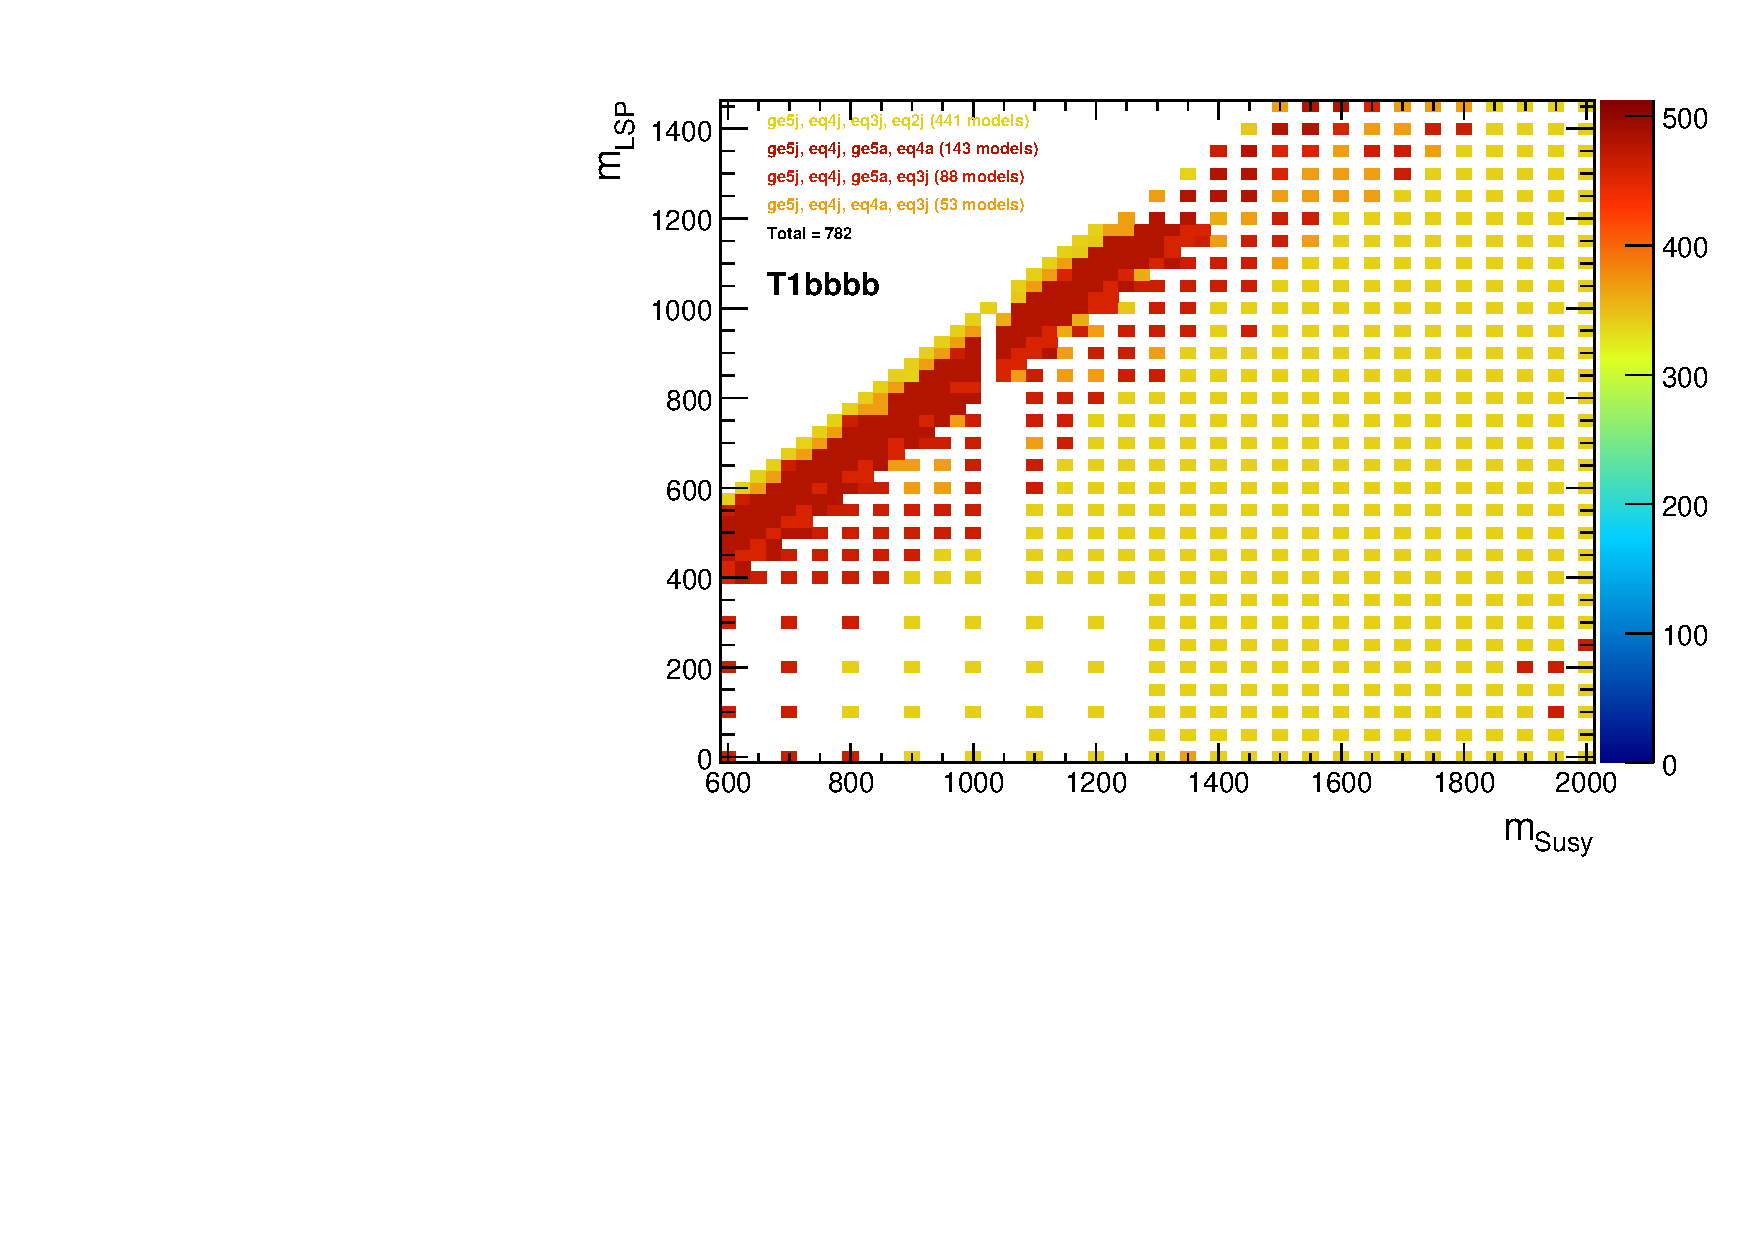
\includegraphics[width=0.5\textwidth]{figures/jetRanking/jetRankingT1bbbb_order2/T1bbbb_bitMap}} ~~
    \subfigure[T1qqqq]{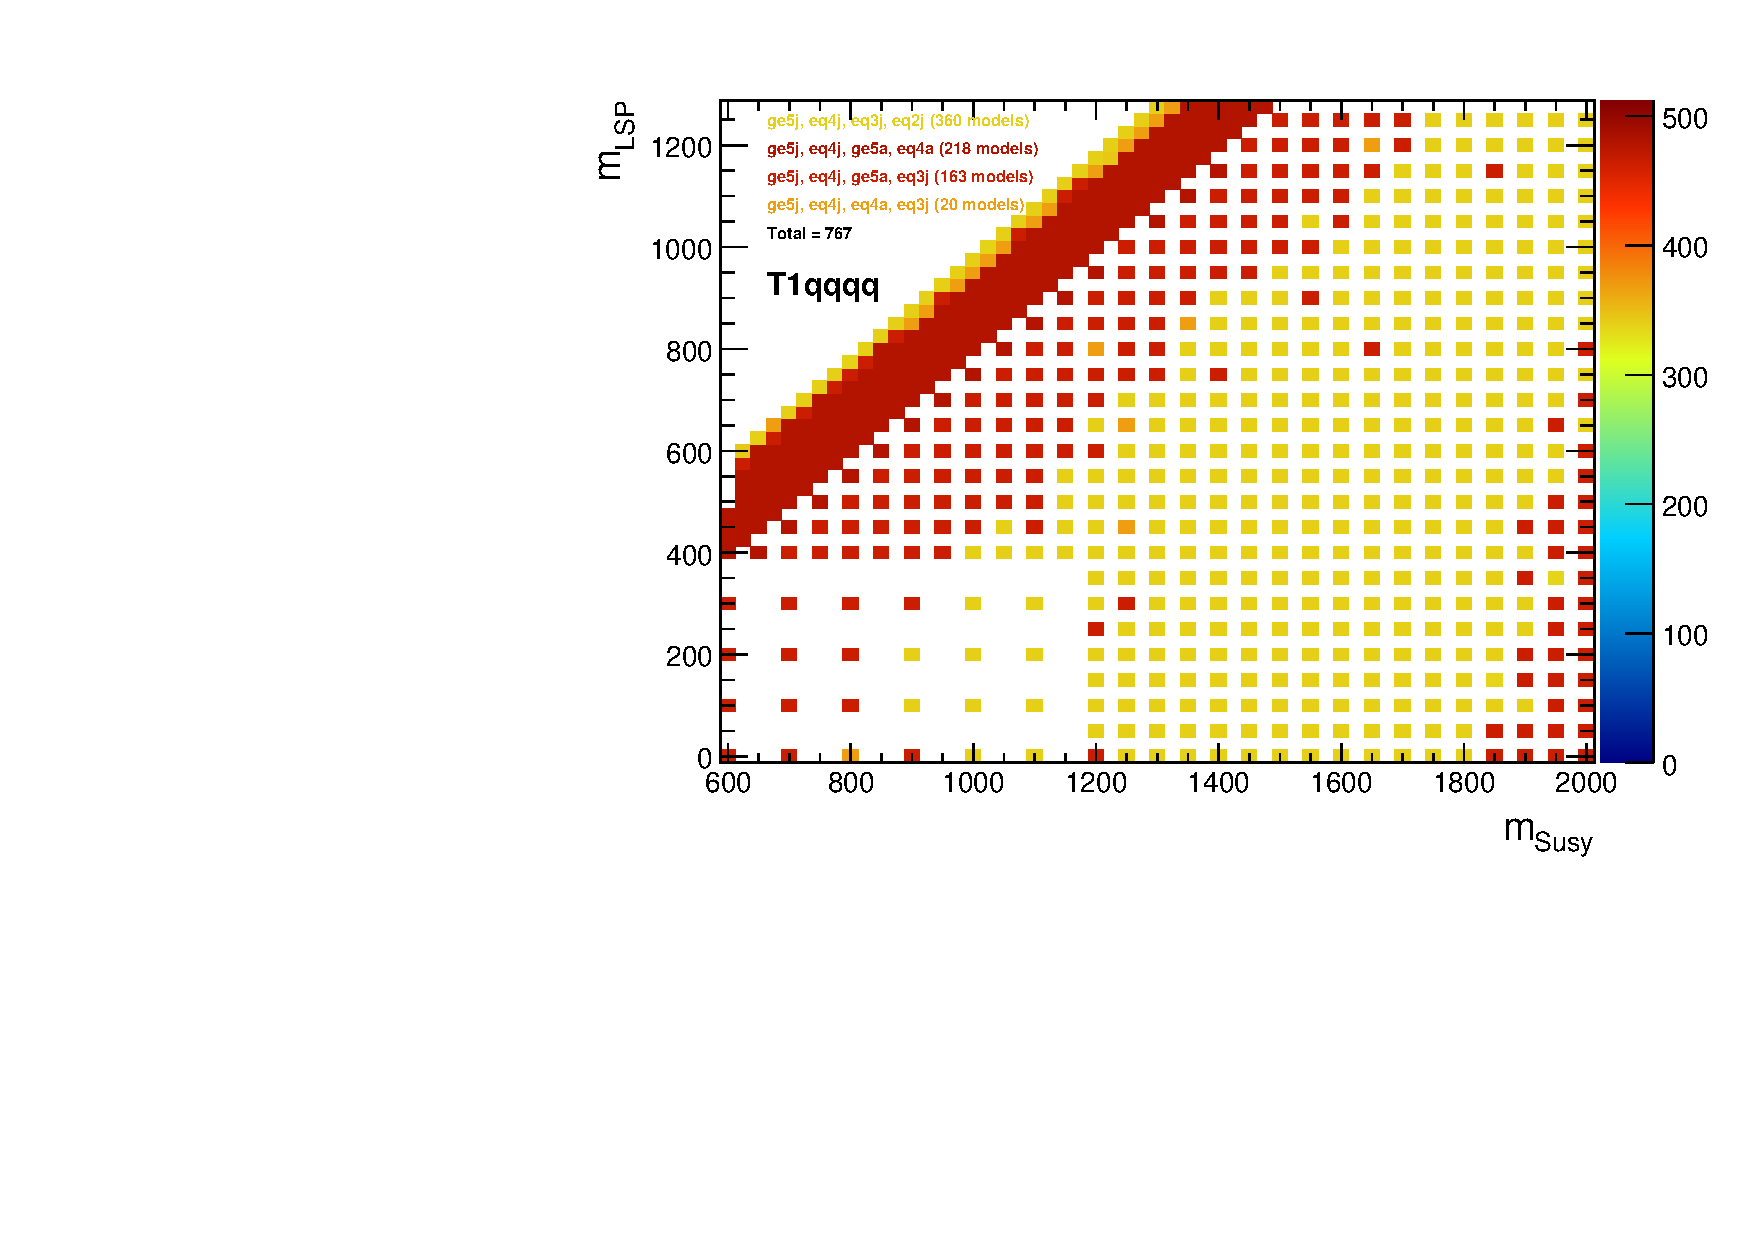
\includegraphics[width=0.5\textwidth]{figures/jetRanking/jetRankingT1qqqq_order2/T1qqqq_bitMap}} \\
    \subfigure[T1tttt]{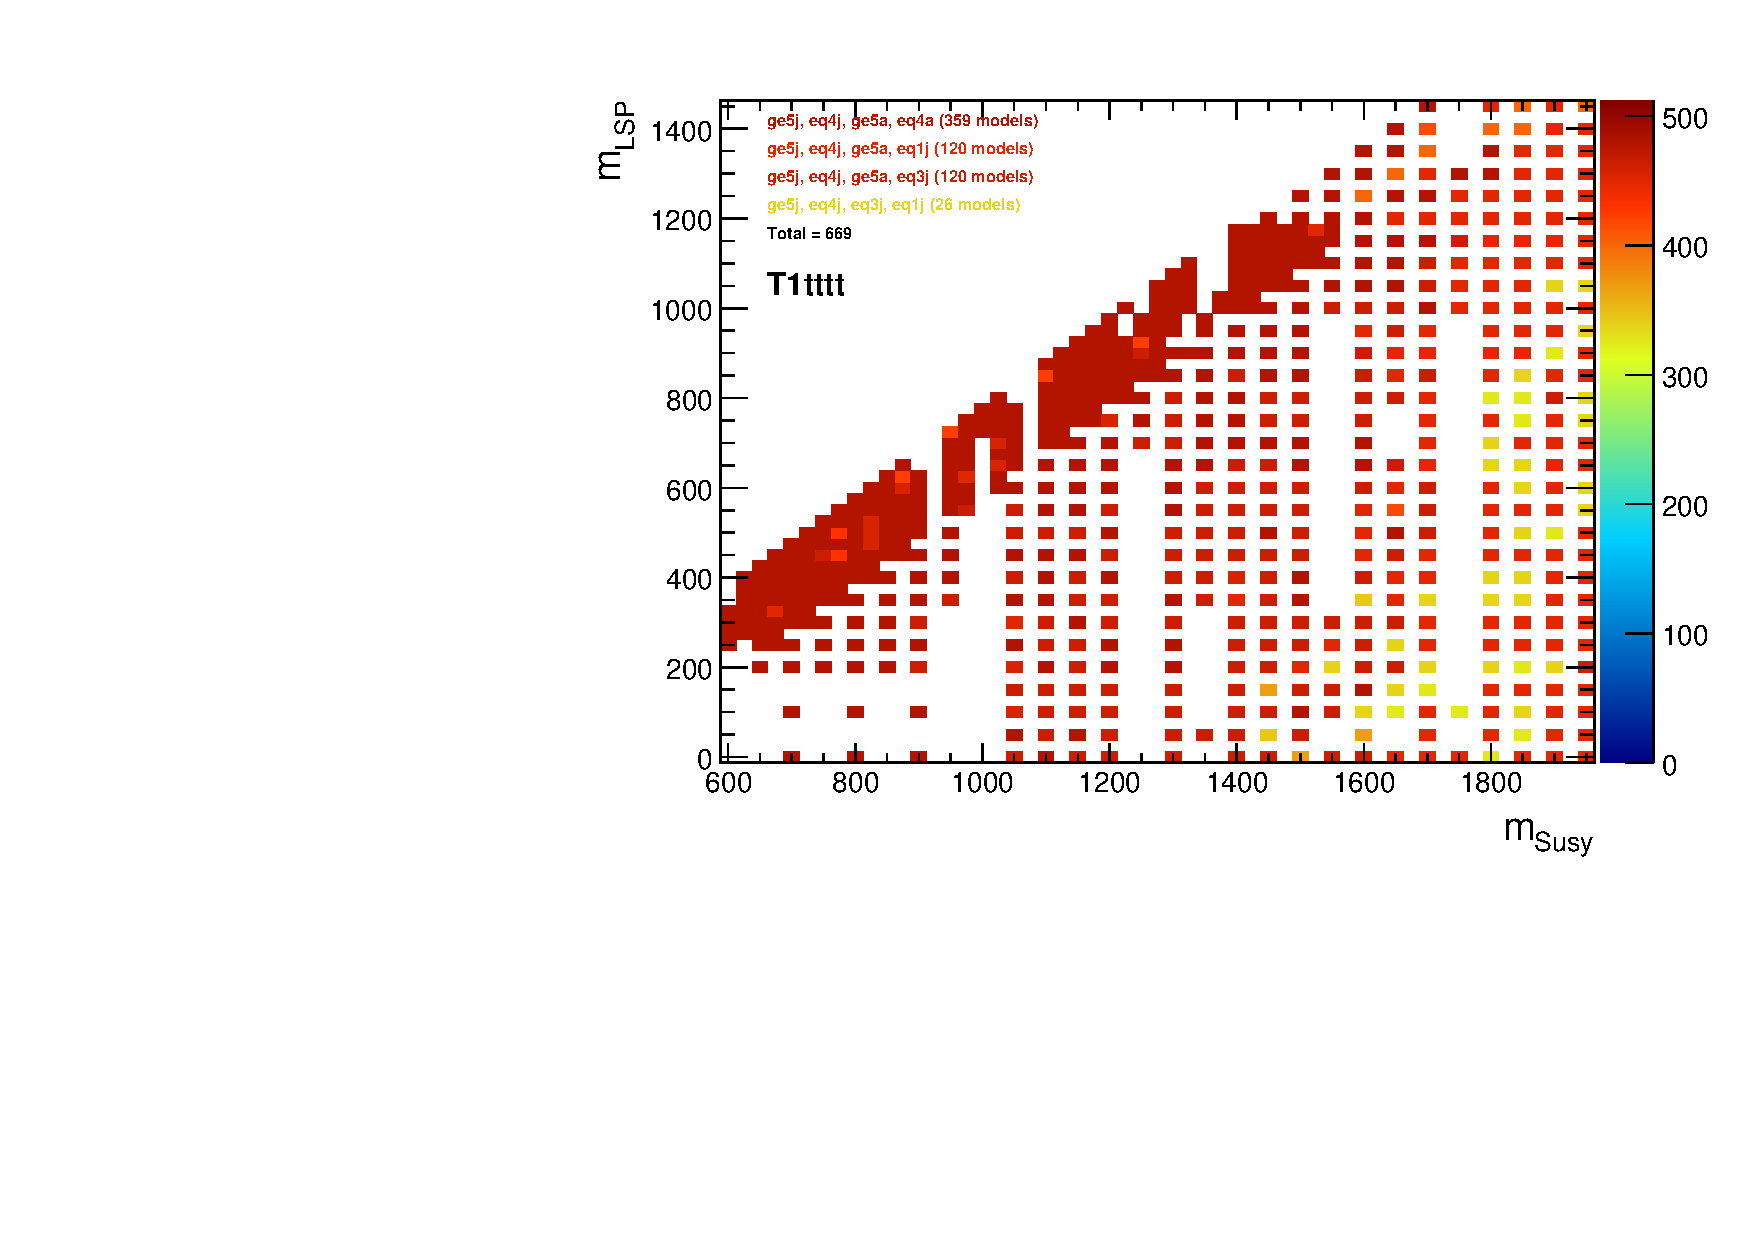
\includegraphics[width=0.5\textwidth]{figures/jetRanking/jetRankingT1tttt_order2/T1tttt_bitMap}}
  \end{center}
\end{figure}

\begin{figure}
  \caption{Ranking of each jet category across the mass plane for the T1bbbb model
  \label{fig:rankingT1bbbb}}
  \begin{center}    
    \subfigure[ge5j]{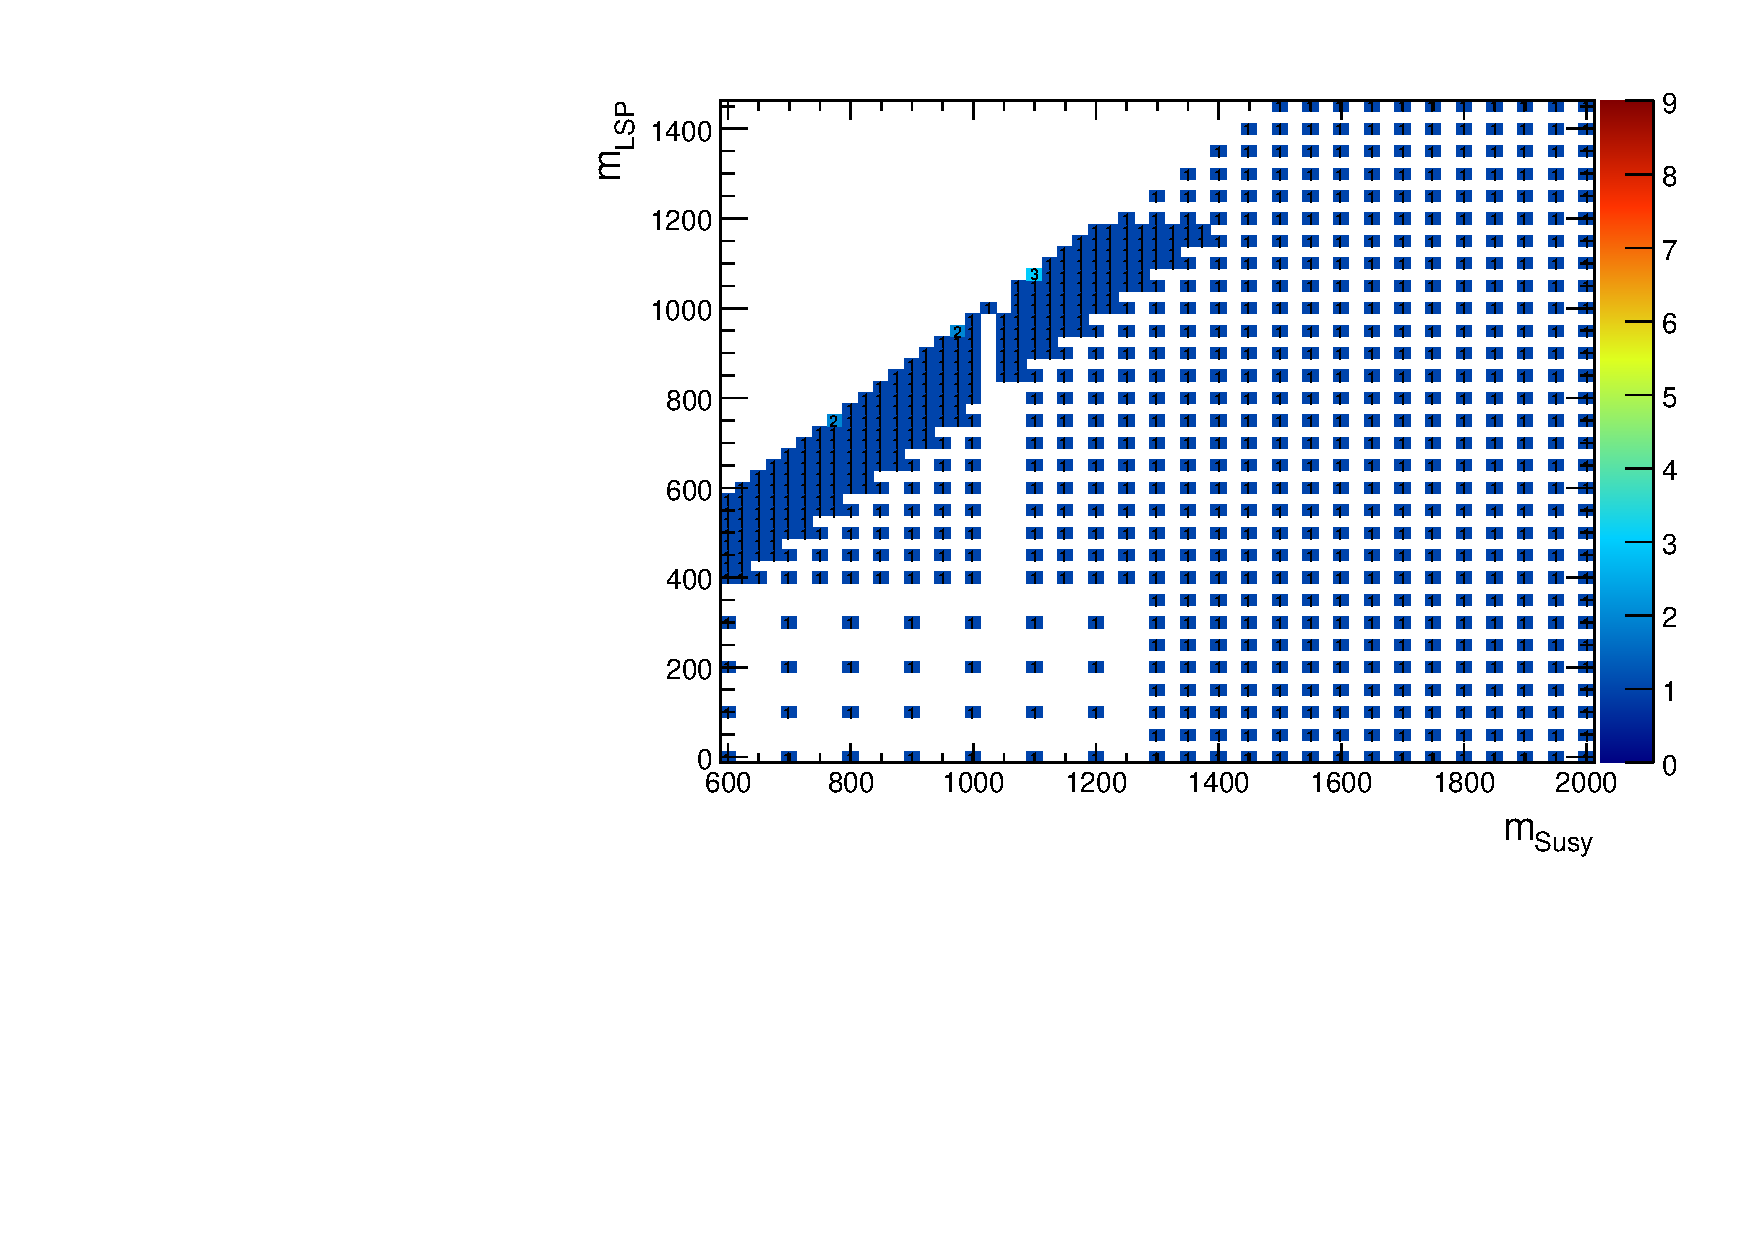
\includegraphics[width=0.33\textwidth]{figures/jetRanking/jetRankingT1bbbb_order2/T1bbbb_ge5j}} ~~
    \subfigure[ge5a]{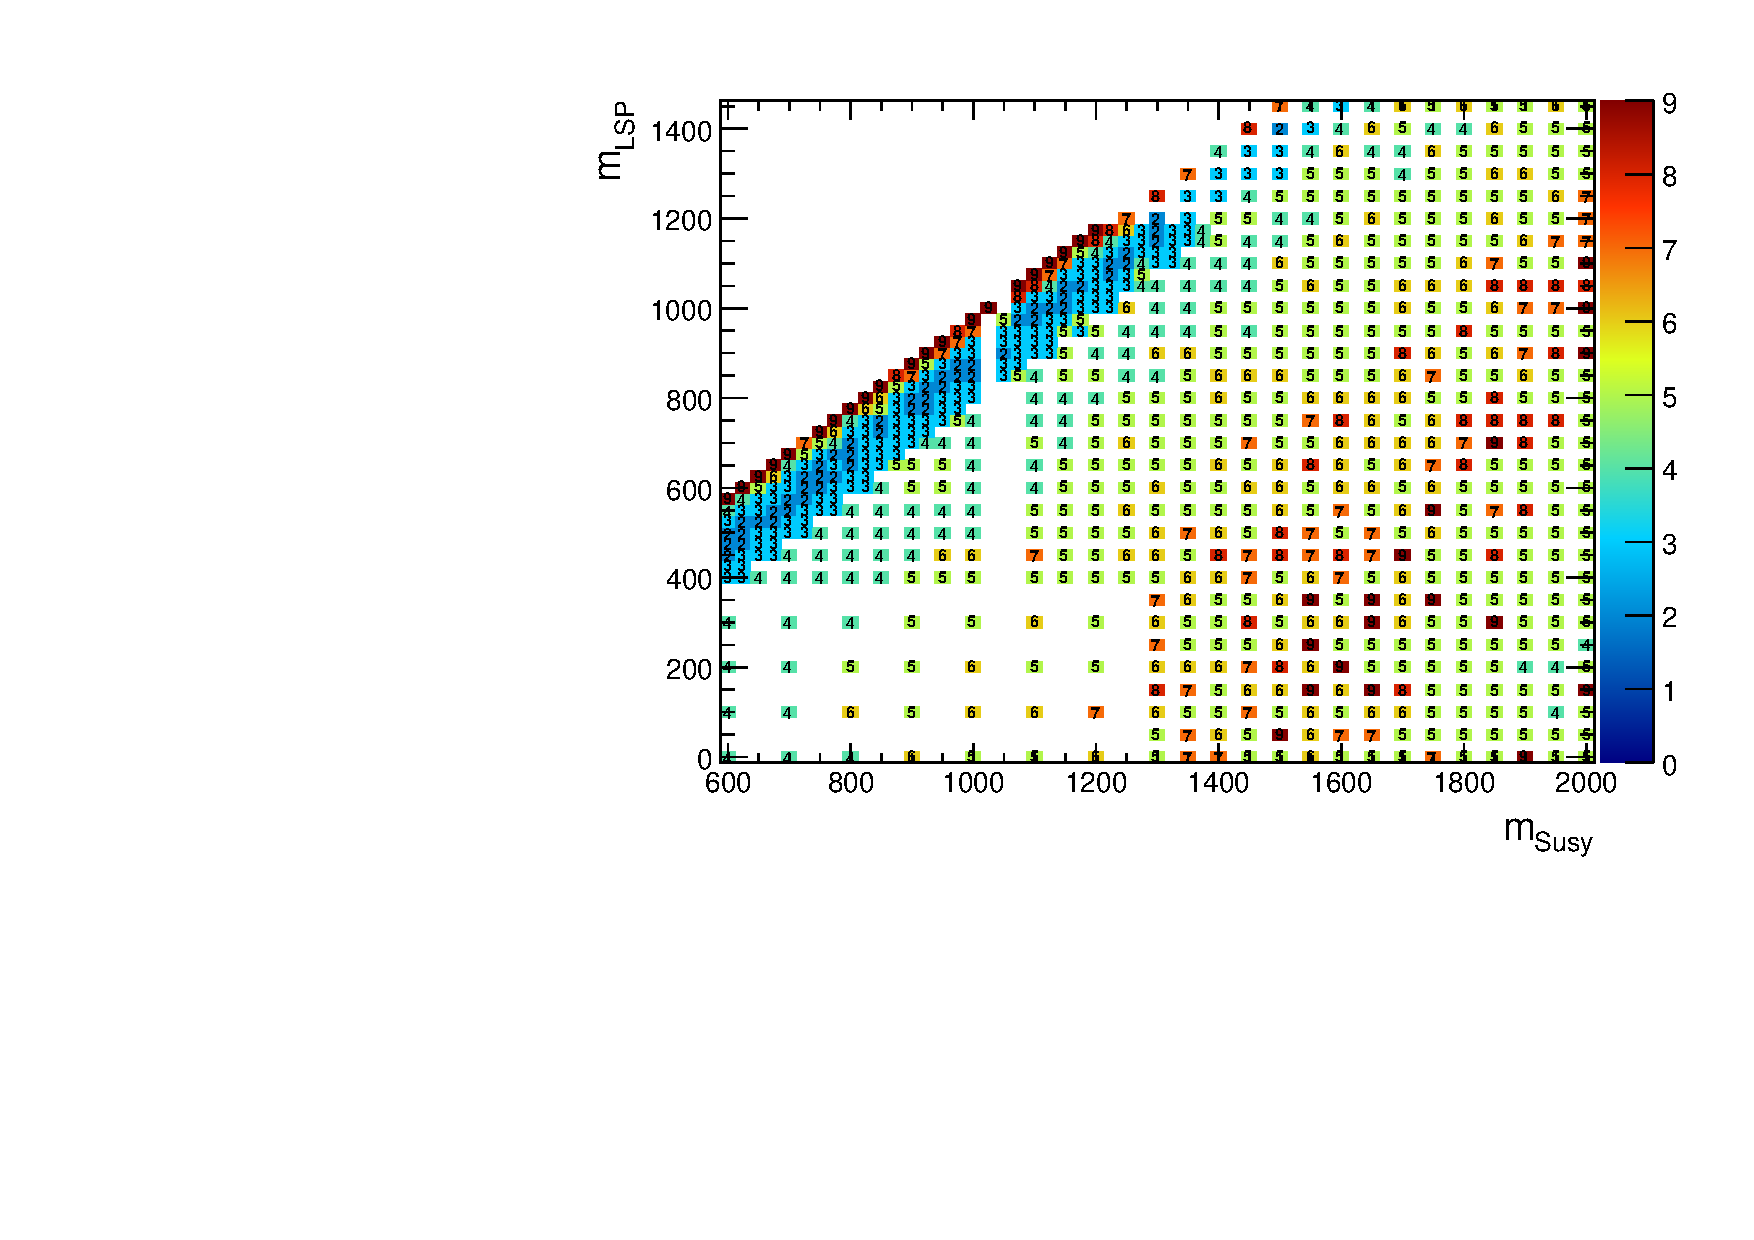
\includegraphics[width=0.33\textwidth]{figures/jetRanking/jetRankingT1bbbb_order2/T1bbbb_ge5a}} ~~
    \subfigure[eq4j]{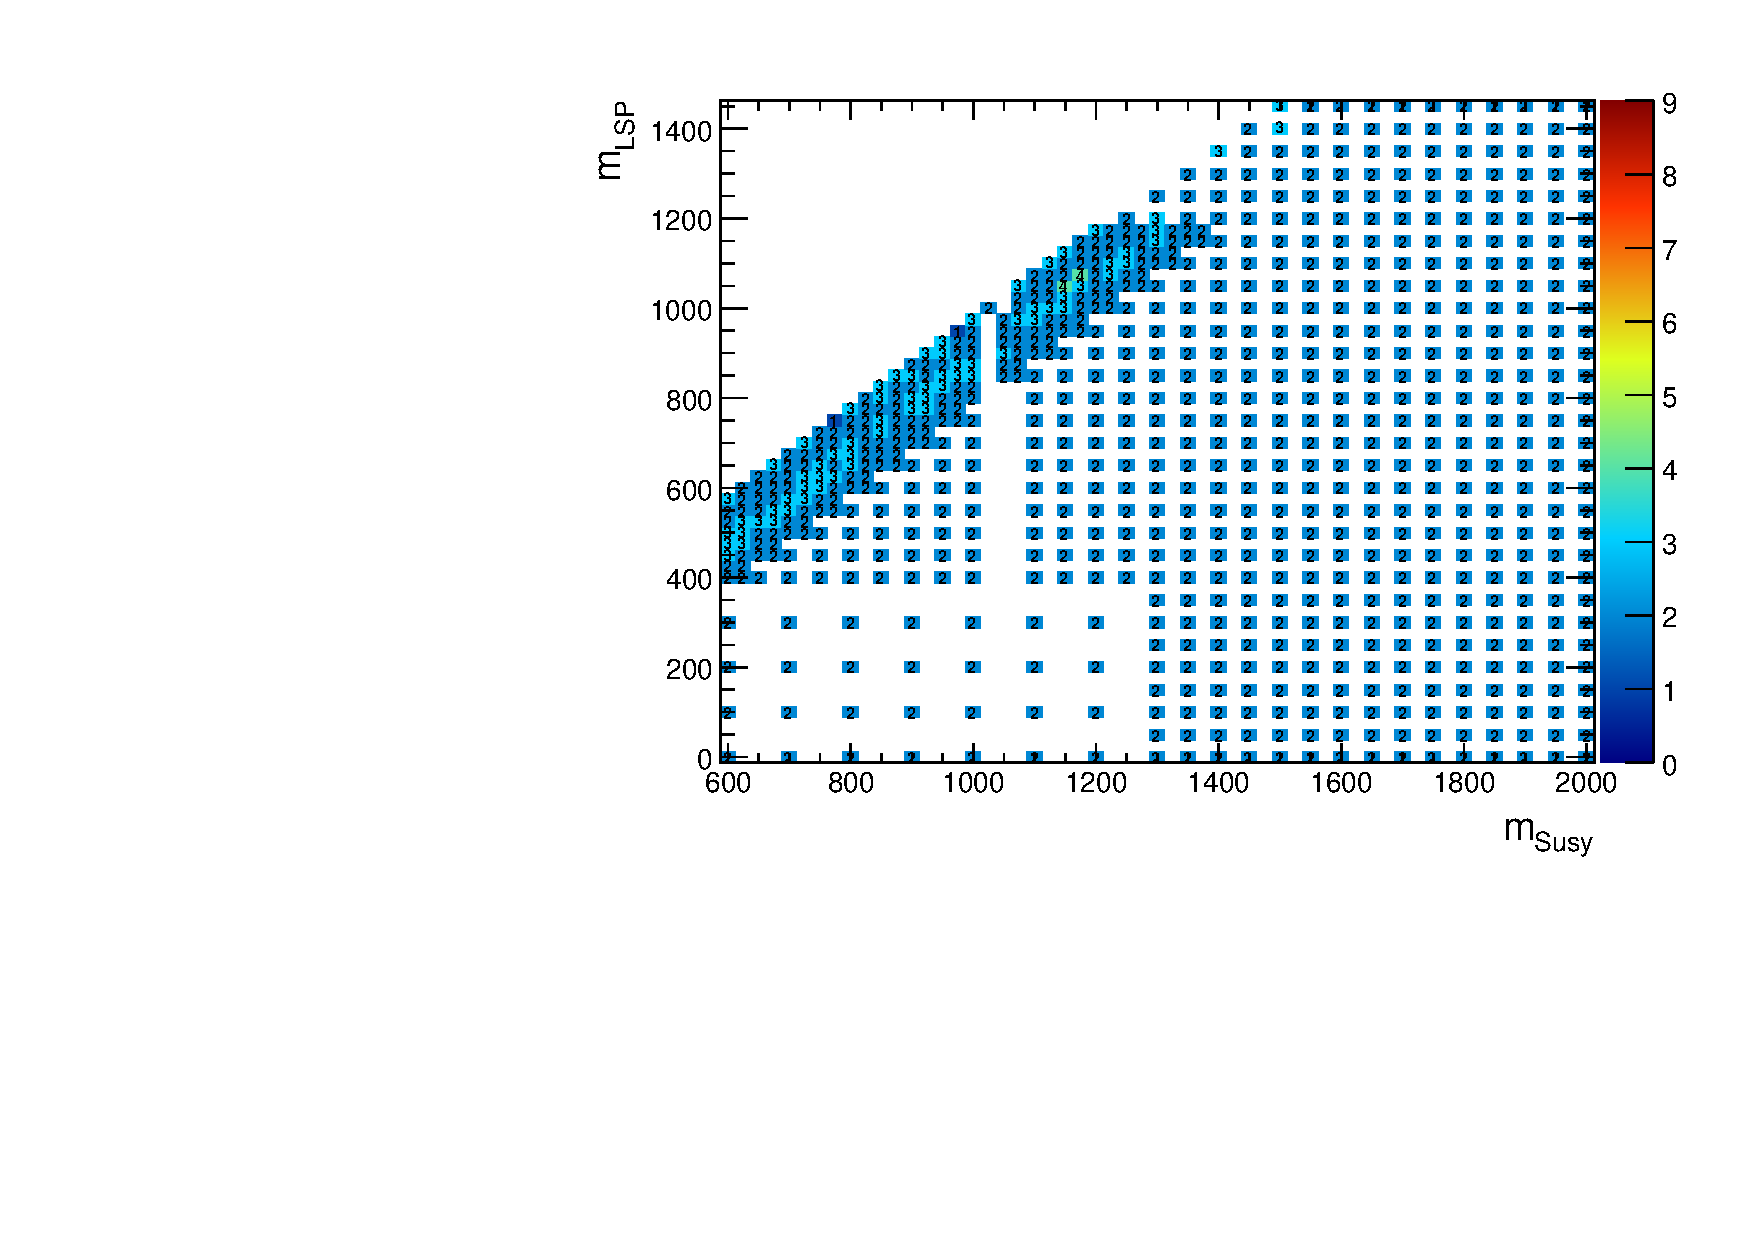
\includegraphics[width=0.33\textwidth]{figures/jetRanking/jetRankingT1bbbb_order2/T1bbbb_eq4j}} \\
    \subfigure[eq4a]{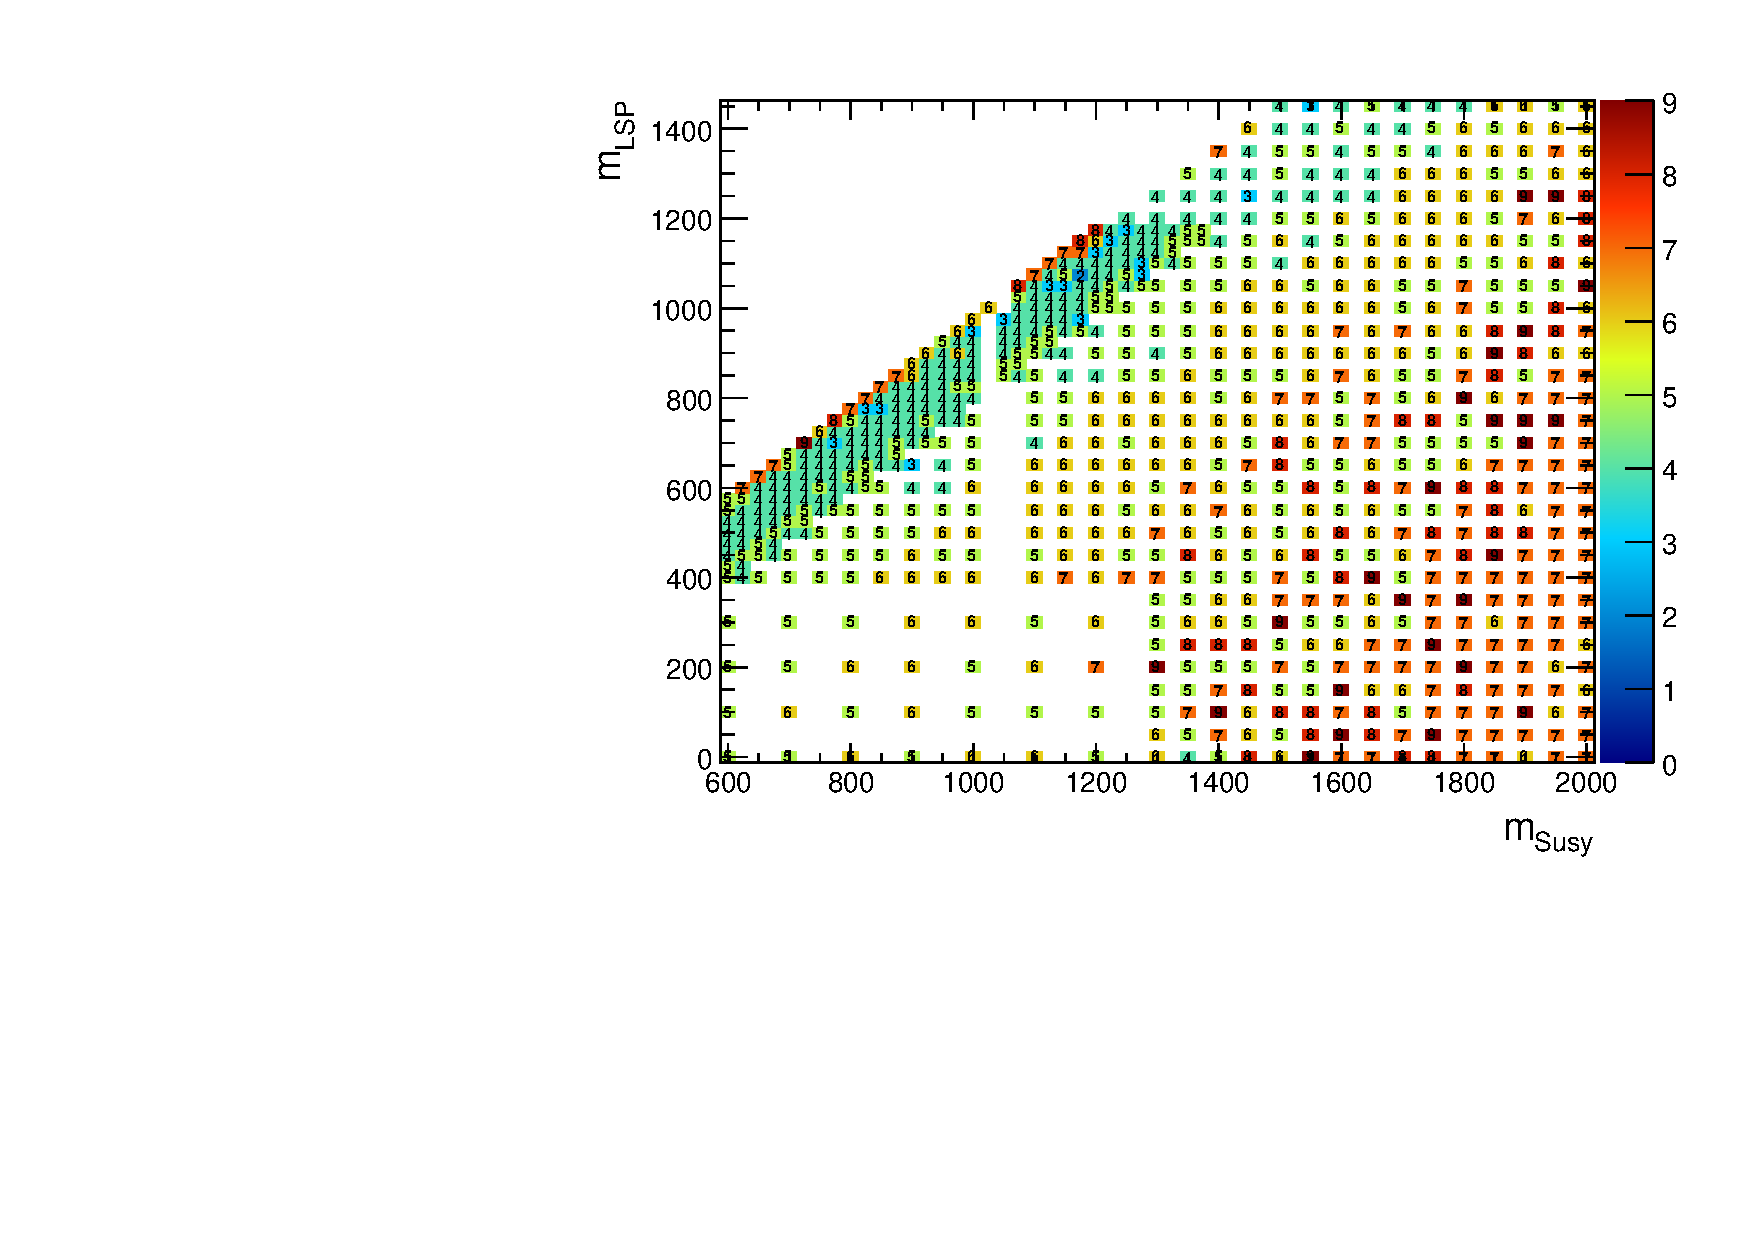
\includegraphics[width=0.33\textwidth]{figures/jetRanking/jetRankingT1bbbb_order2/T1bbbb_eq4a}} ~~
    \subfigure[eq3j]{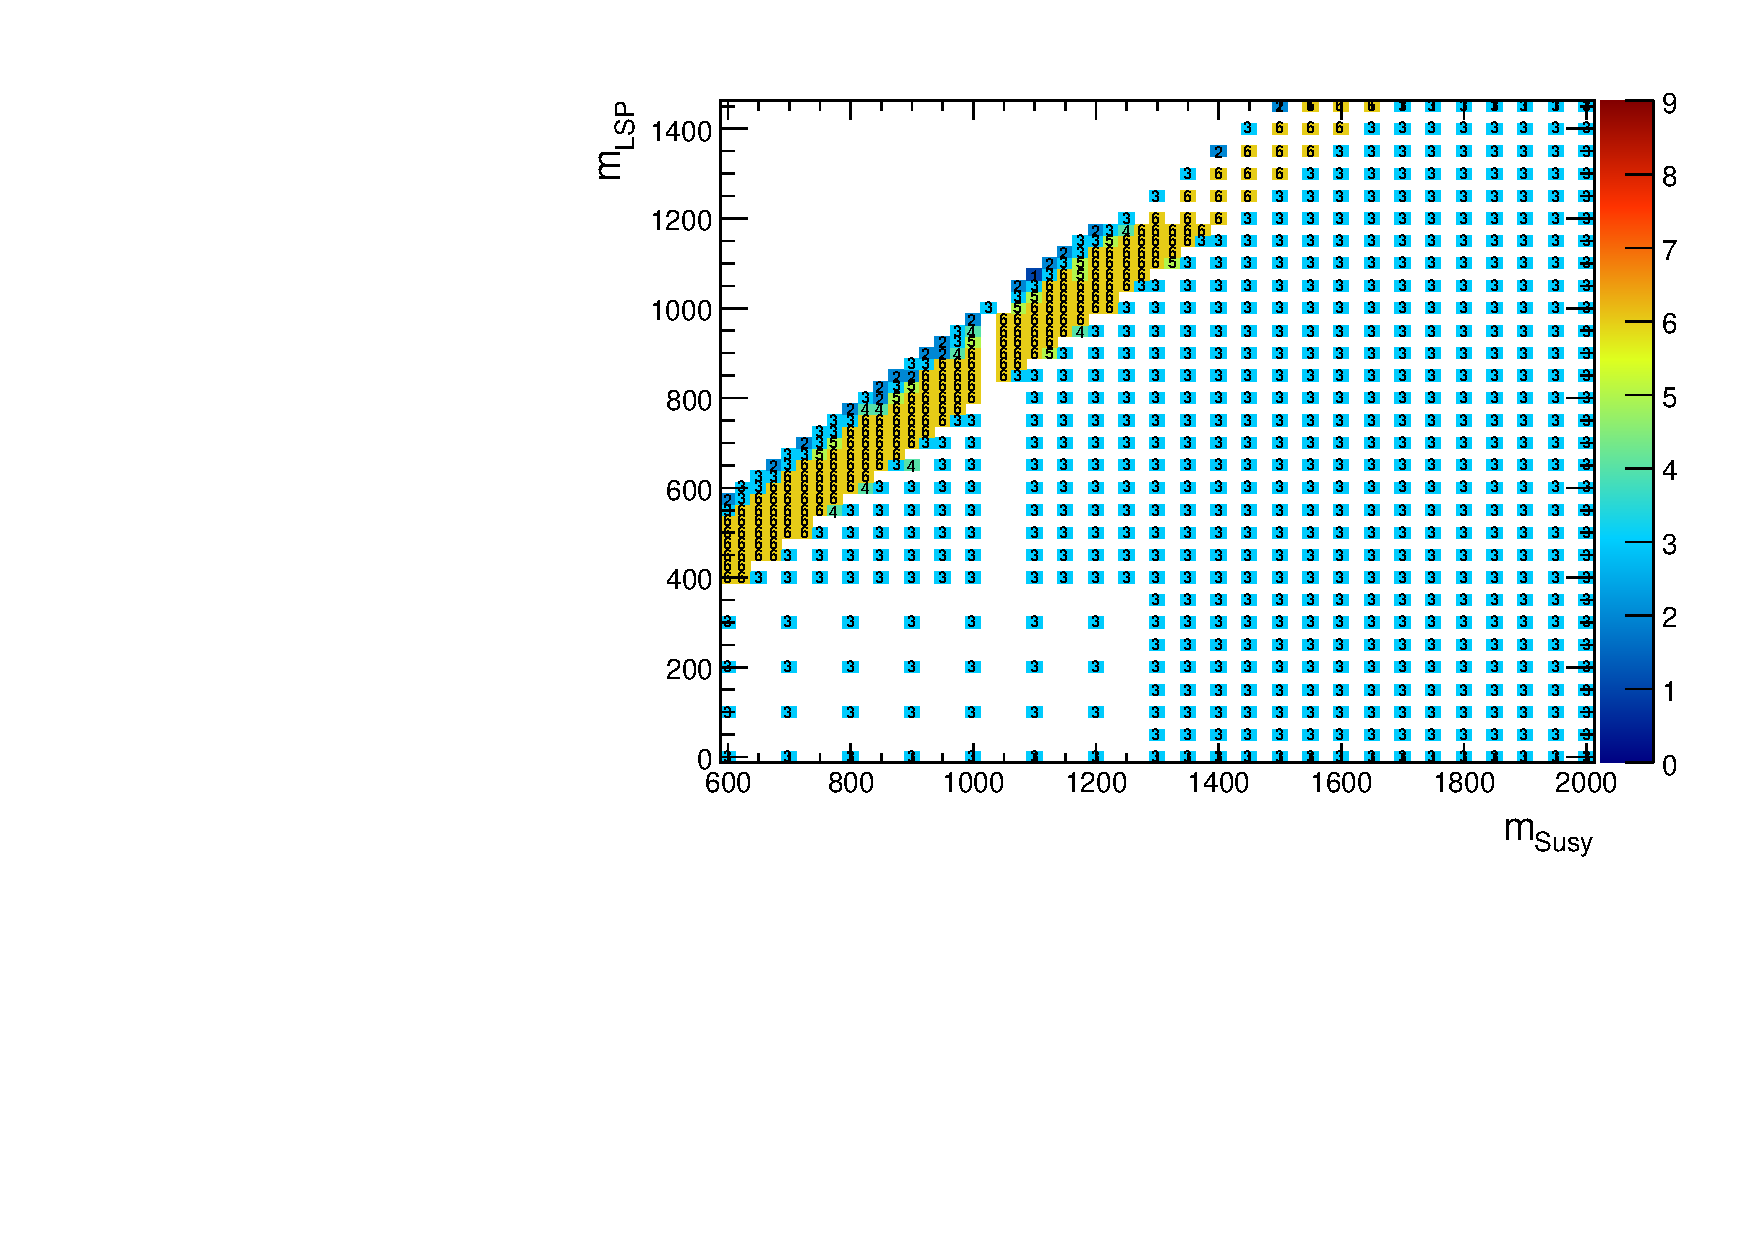
\includegraphics[width=0.33\textwidth]{figures/jetRanking/jetRankingT1bbbb_order2/T1bbbb_eq3j}} ~~
    \subfigure[eq3a]{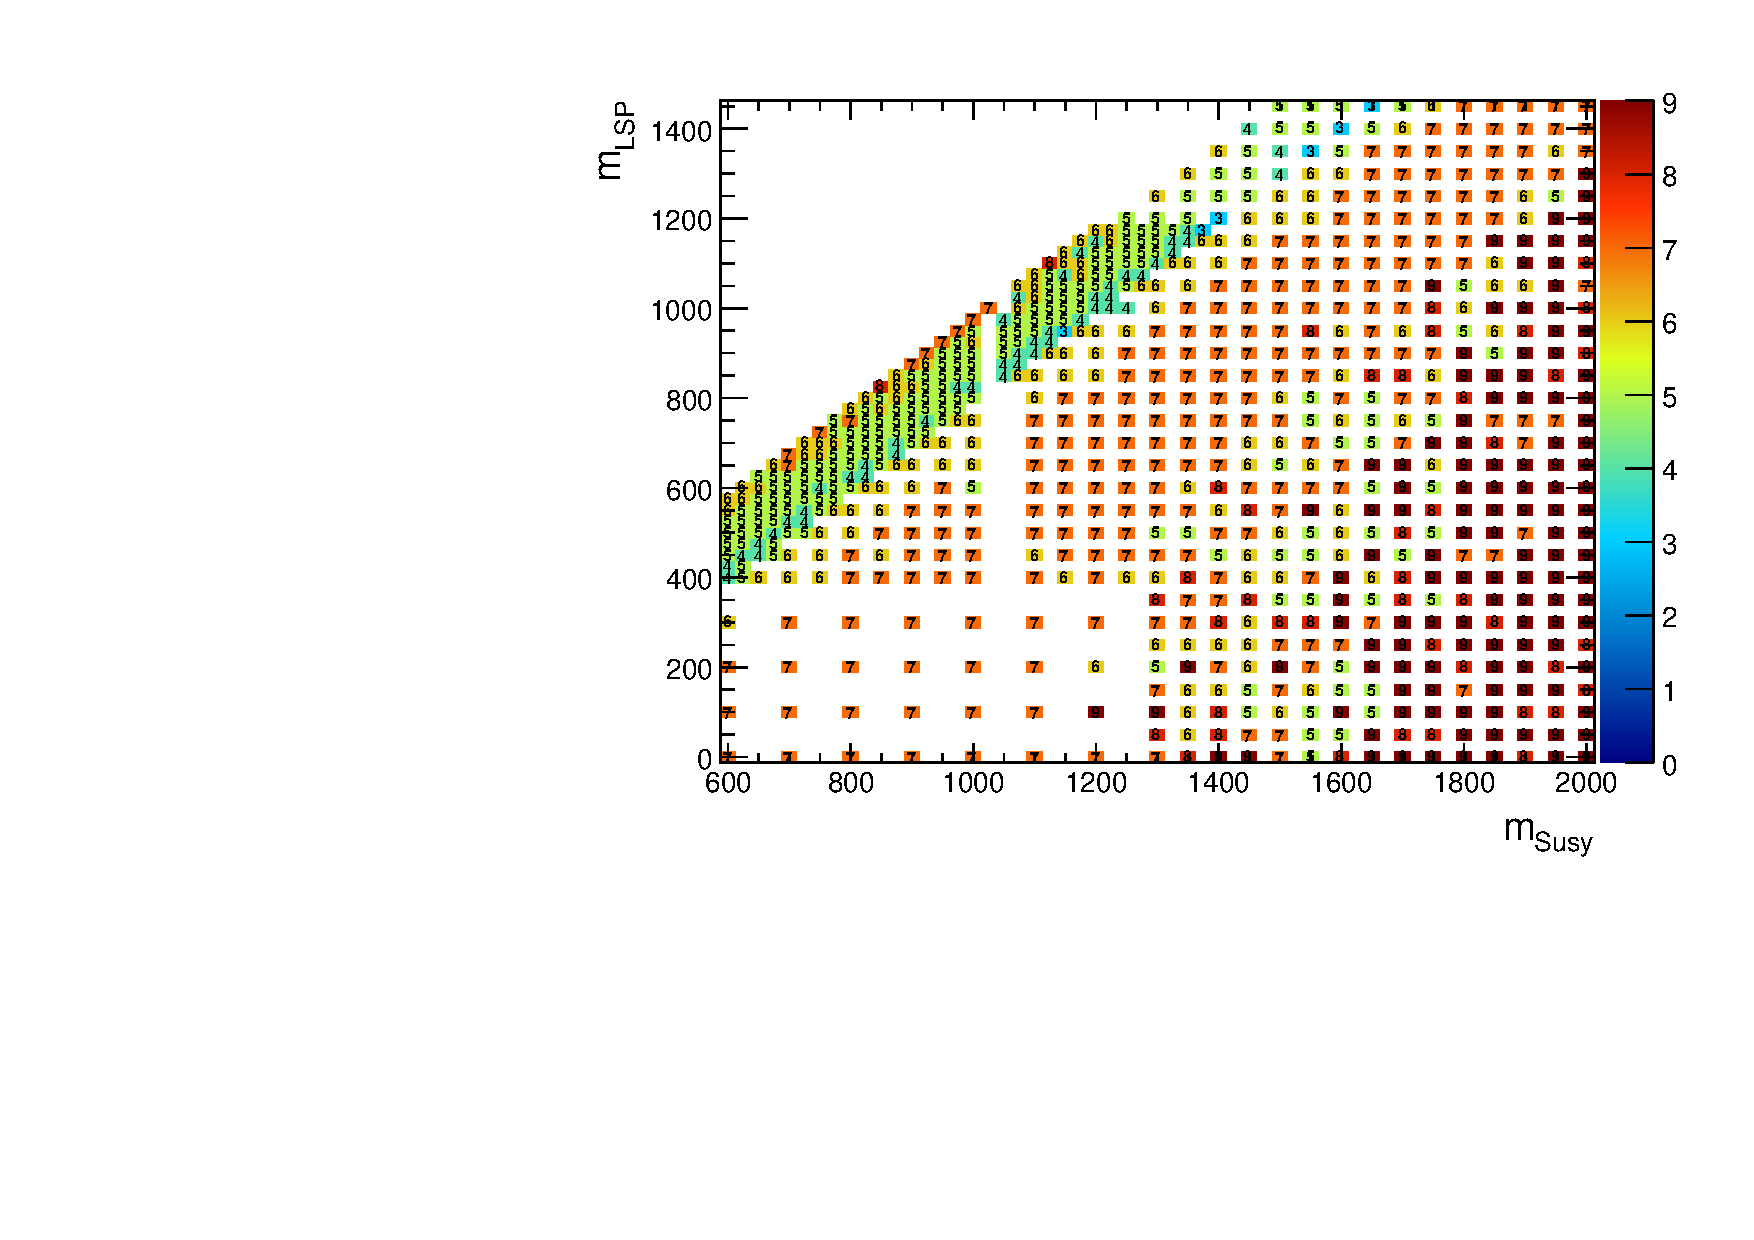
\includegraphics[width=0.33\textwidth]{figures/jetRanking/jetRankingT1bbbb_order2/T1bbbb_eq3a}} \\
    \subfigure[eq2j]{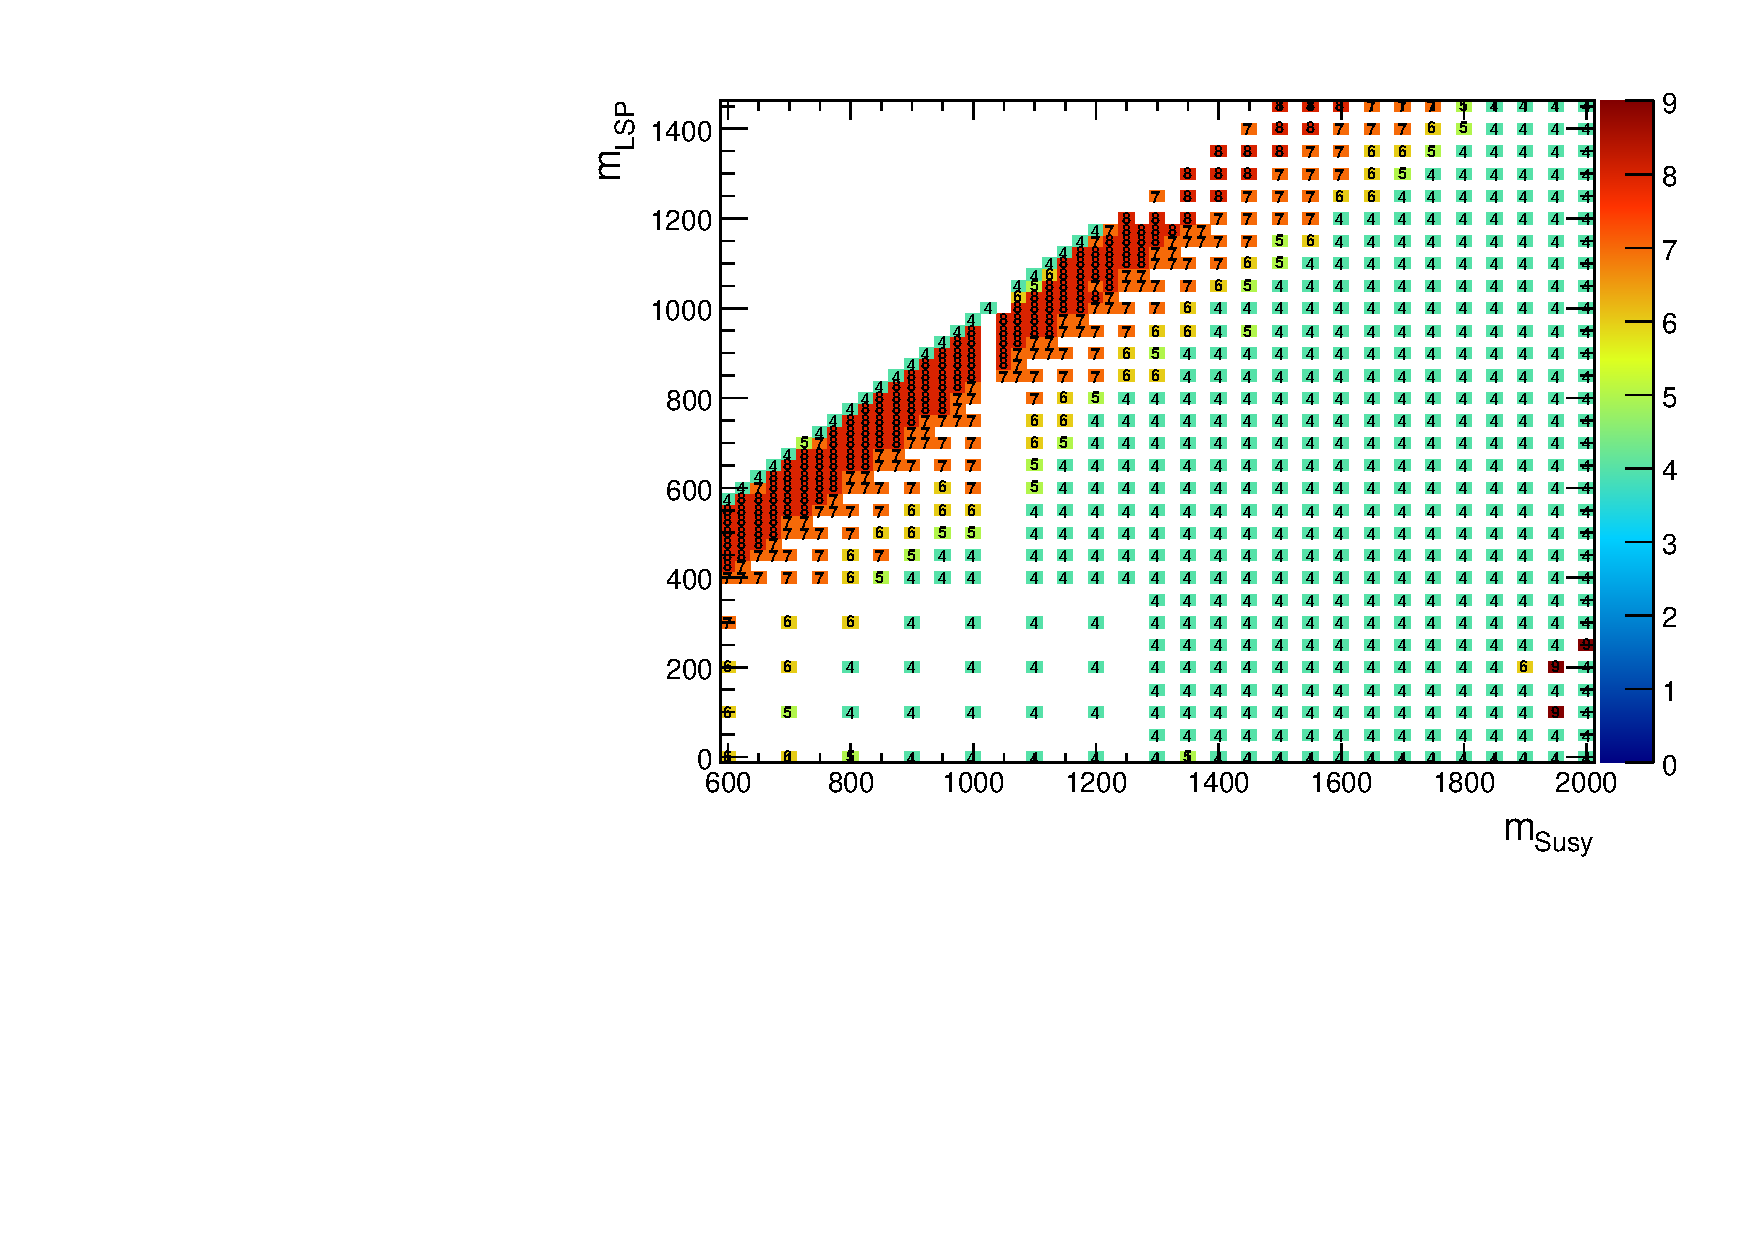
\includegraphics[width=0.33\textwidth]{figures/jetRanking/jetRankingT1bbbb_order2/T1bbbb_eq2j}} ~~
    \subfigure[eq2a]{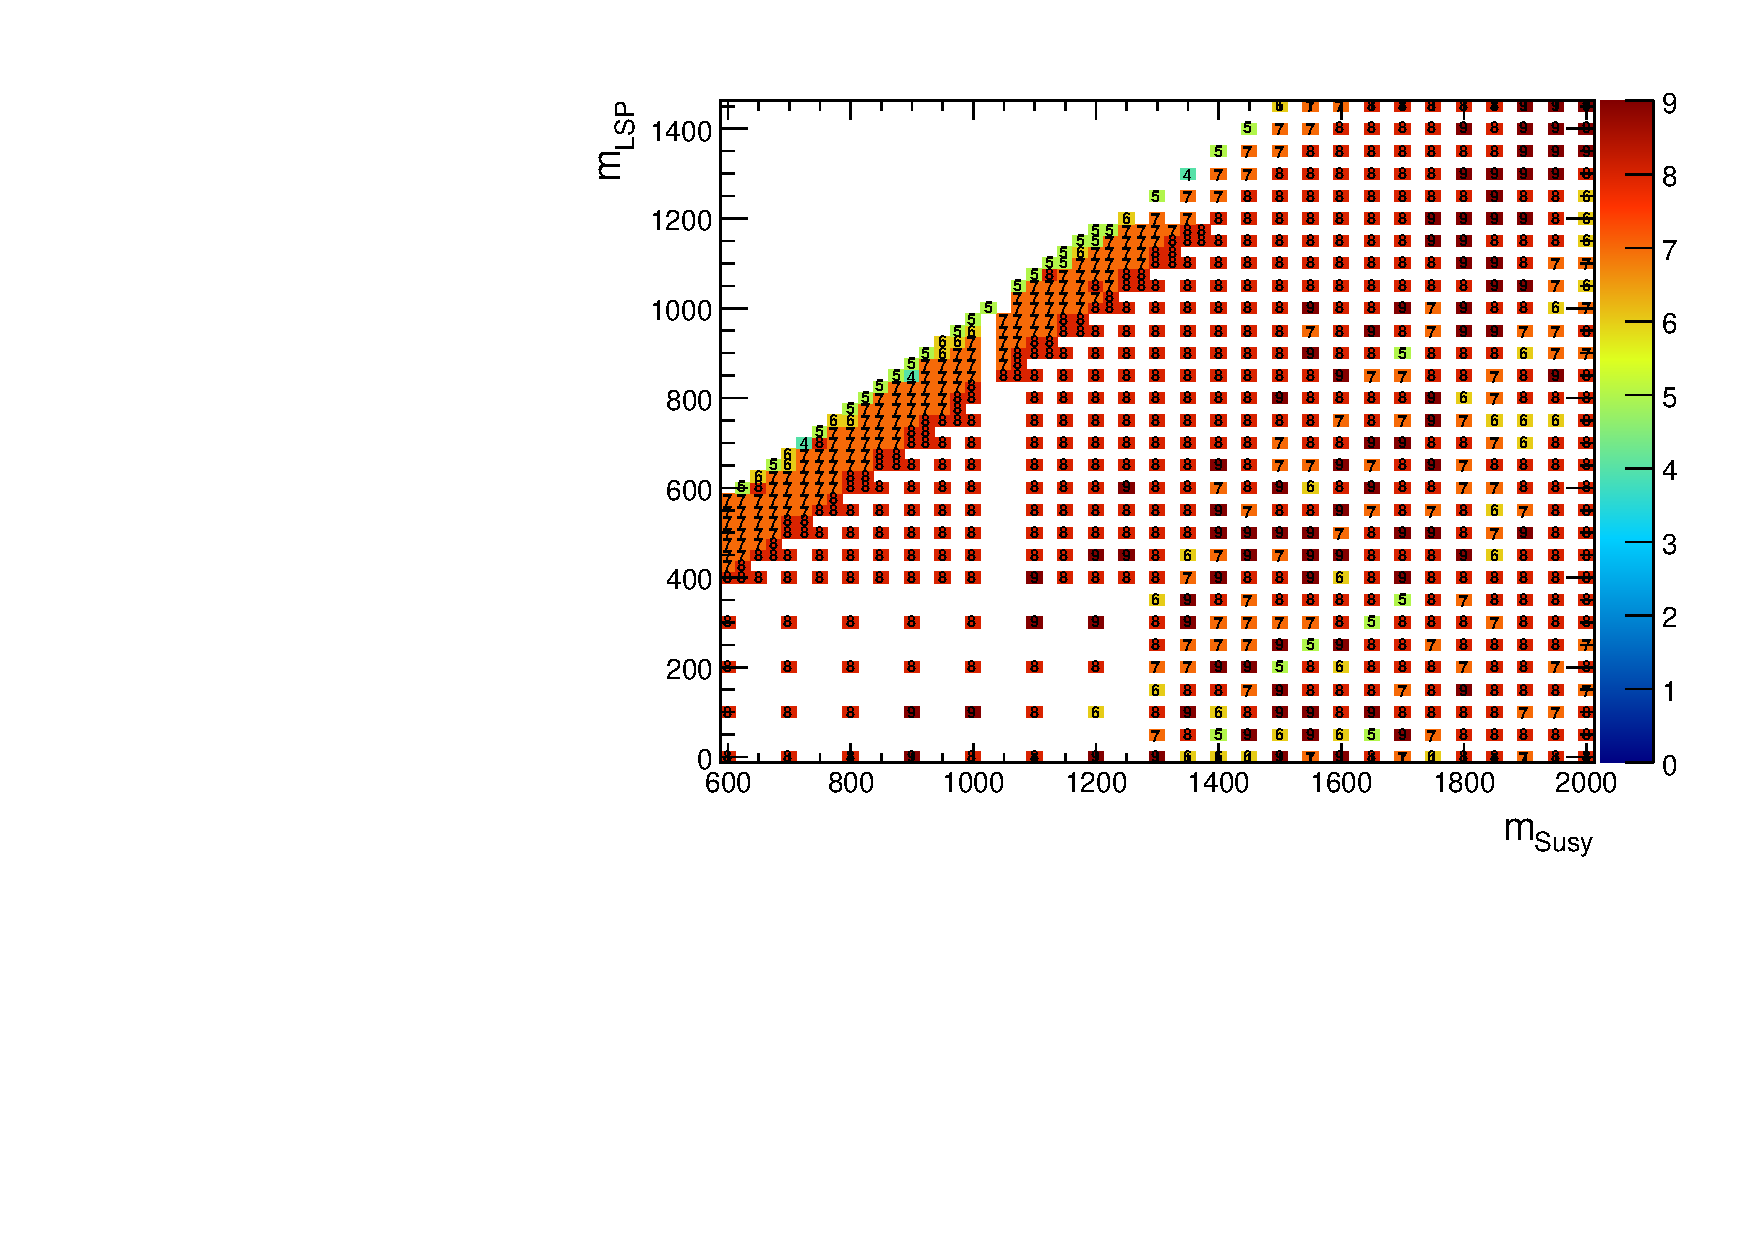
\includegraphics[width=0.33\textwidth]{figures/jetRanking/jetRankingT1bbbb_order2/T1bbbb_eq2a}} ~~
    \subfigure[eq1j]{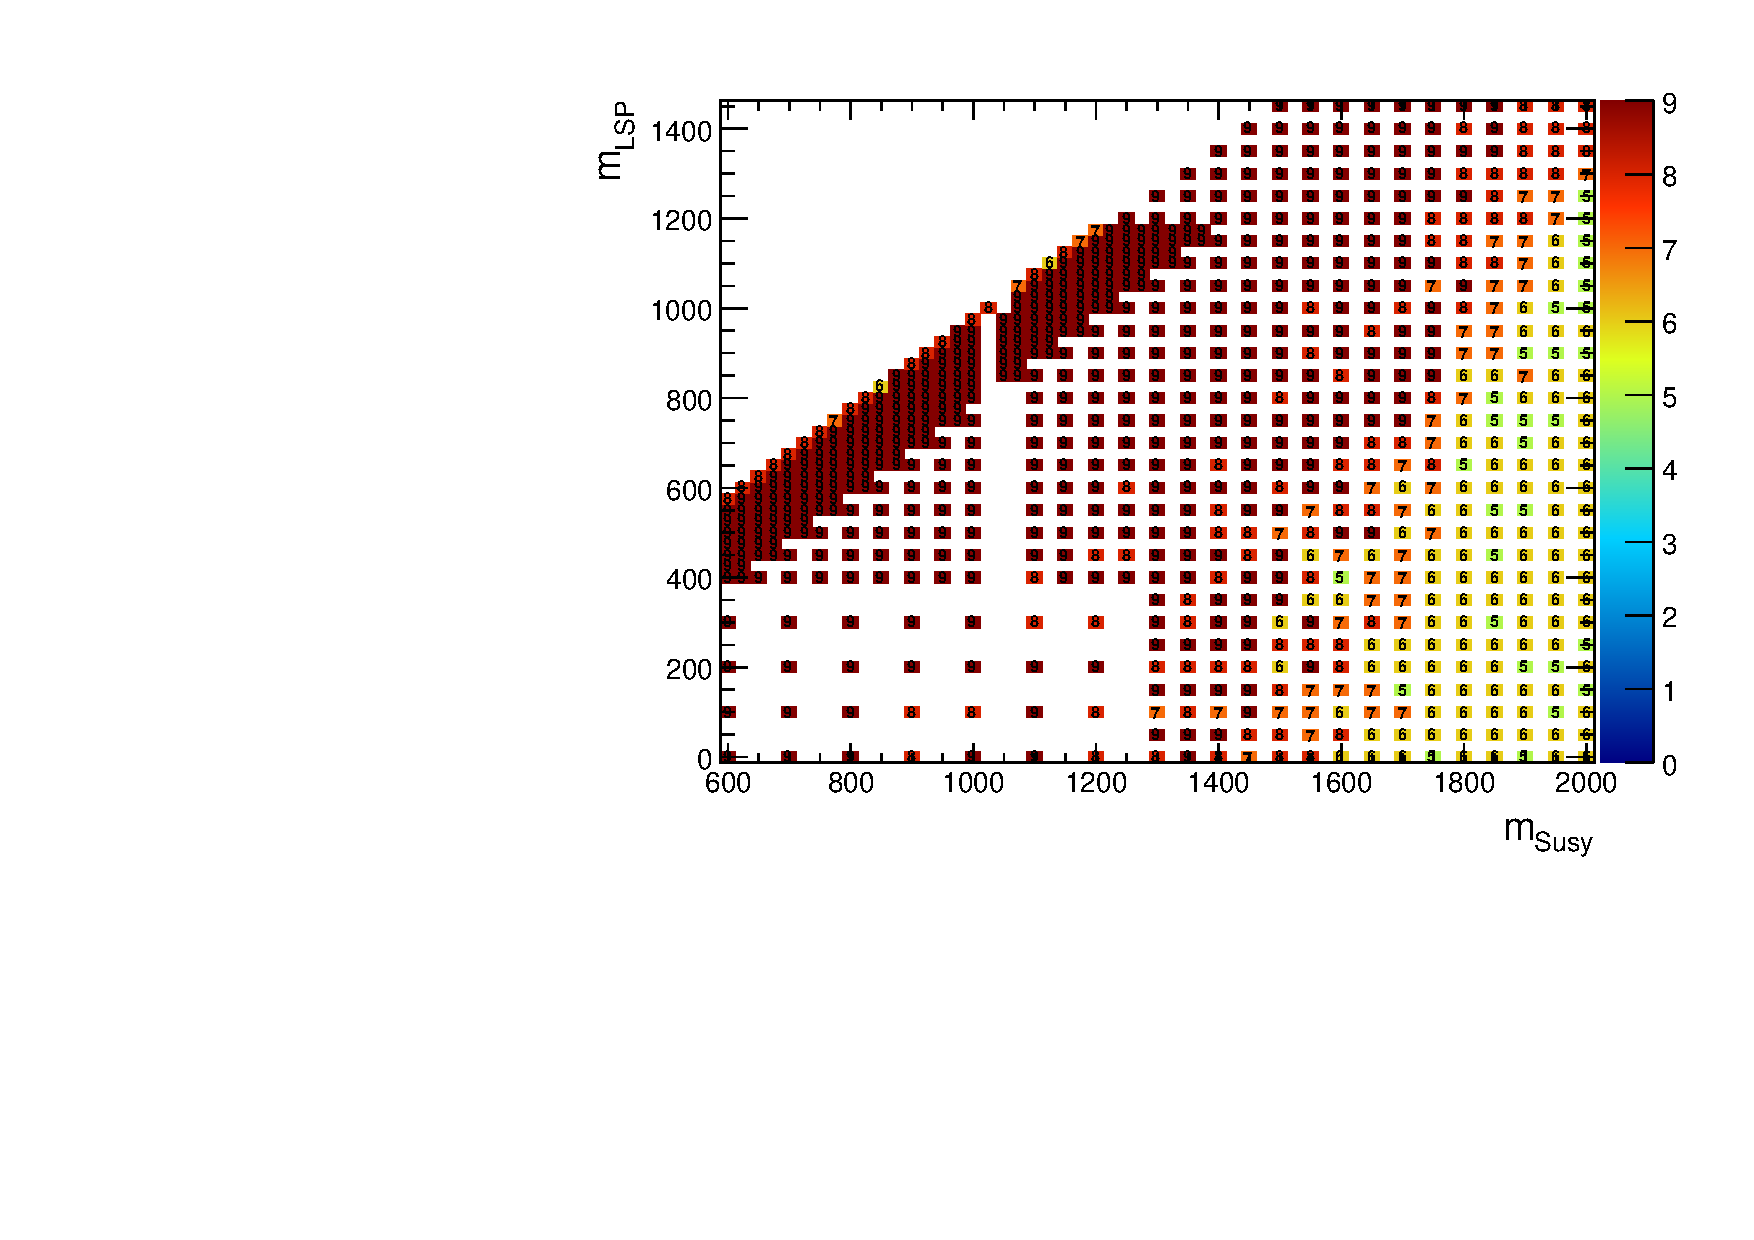
\includegraphics[width=0.33\textwidth]{figures/jetRanking/jetRankingT1bbbb_order2/T1bbbb_eq1j}} \\
  \end{center}
\end{figure}
\begin{figure}
  \caption{Ranking of each jet category across the mass plane for the T1qqqq model
  \label{fig:rankingT1qqqq}}
  \begin{center}    
    \subfigure[ge5j]{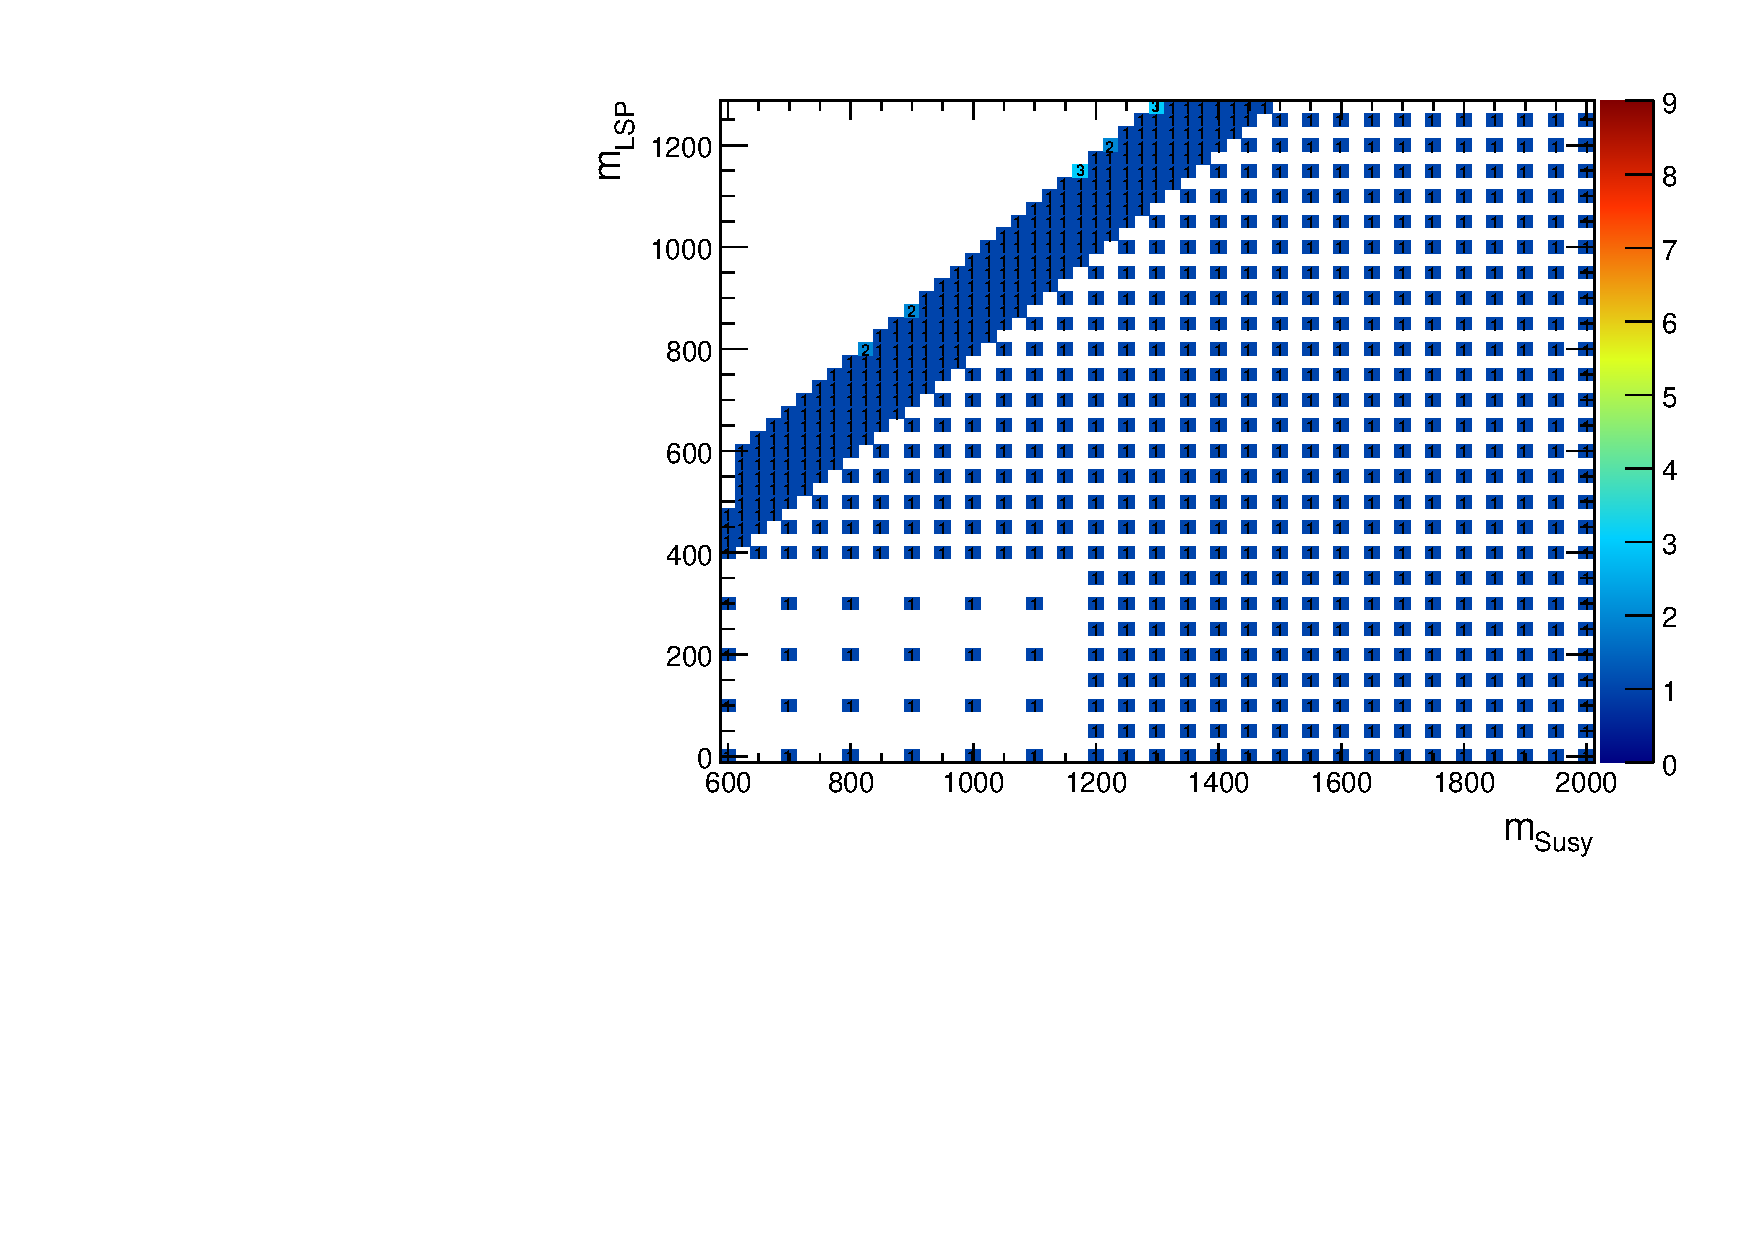
\includegraphics[width=0.33\textwidth]{figures/jetRanking/jetRankingT1qqqq_order2/T1qqqq_ge5j}} ~~
    \subfigure[ge5a]{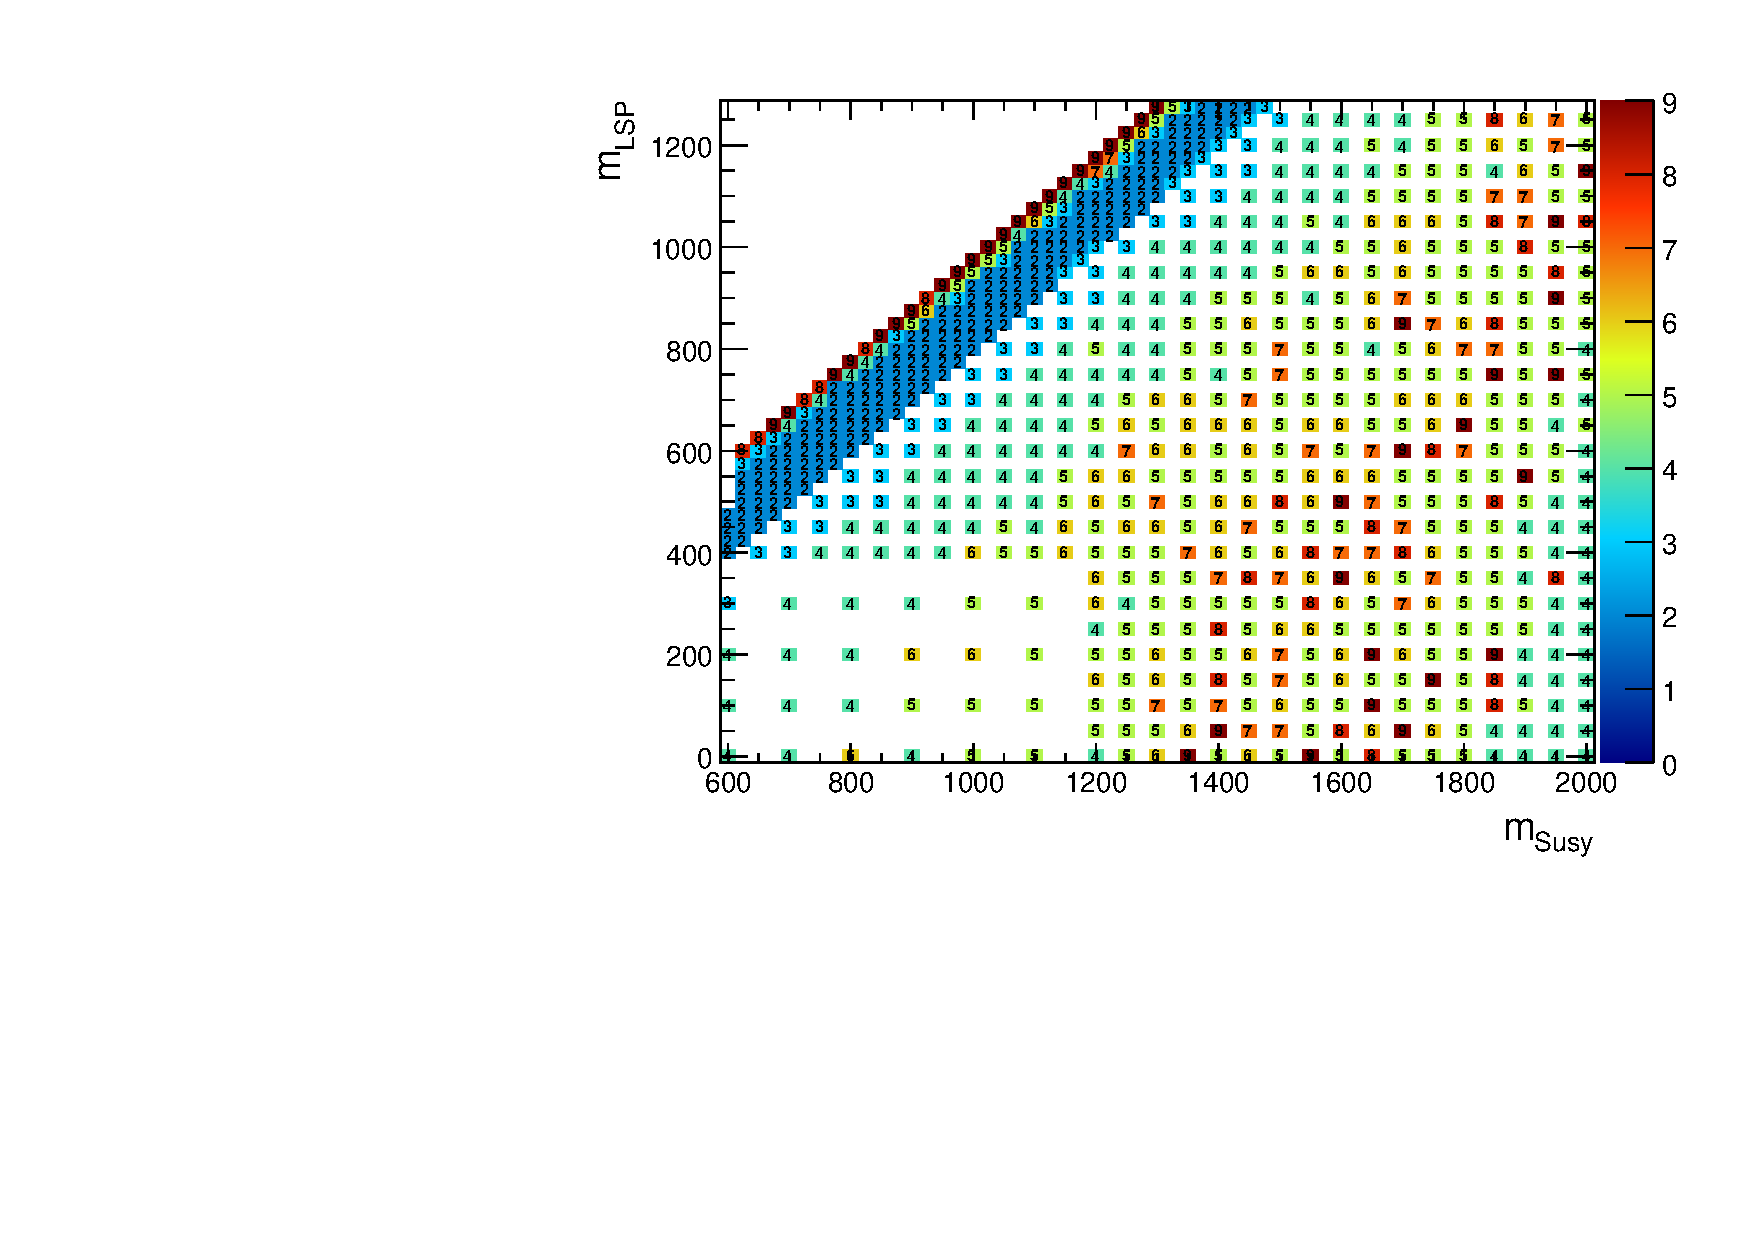
\includegraphics[width=0.33\textwidth]{figures/jetRanking/jetRankingT1qqqq_order2/T1qqqq_ge5a}} ~~
    \subfigure[eq4j]{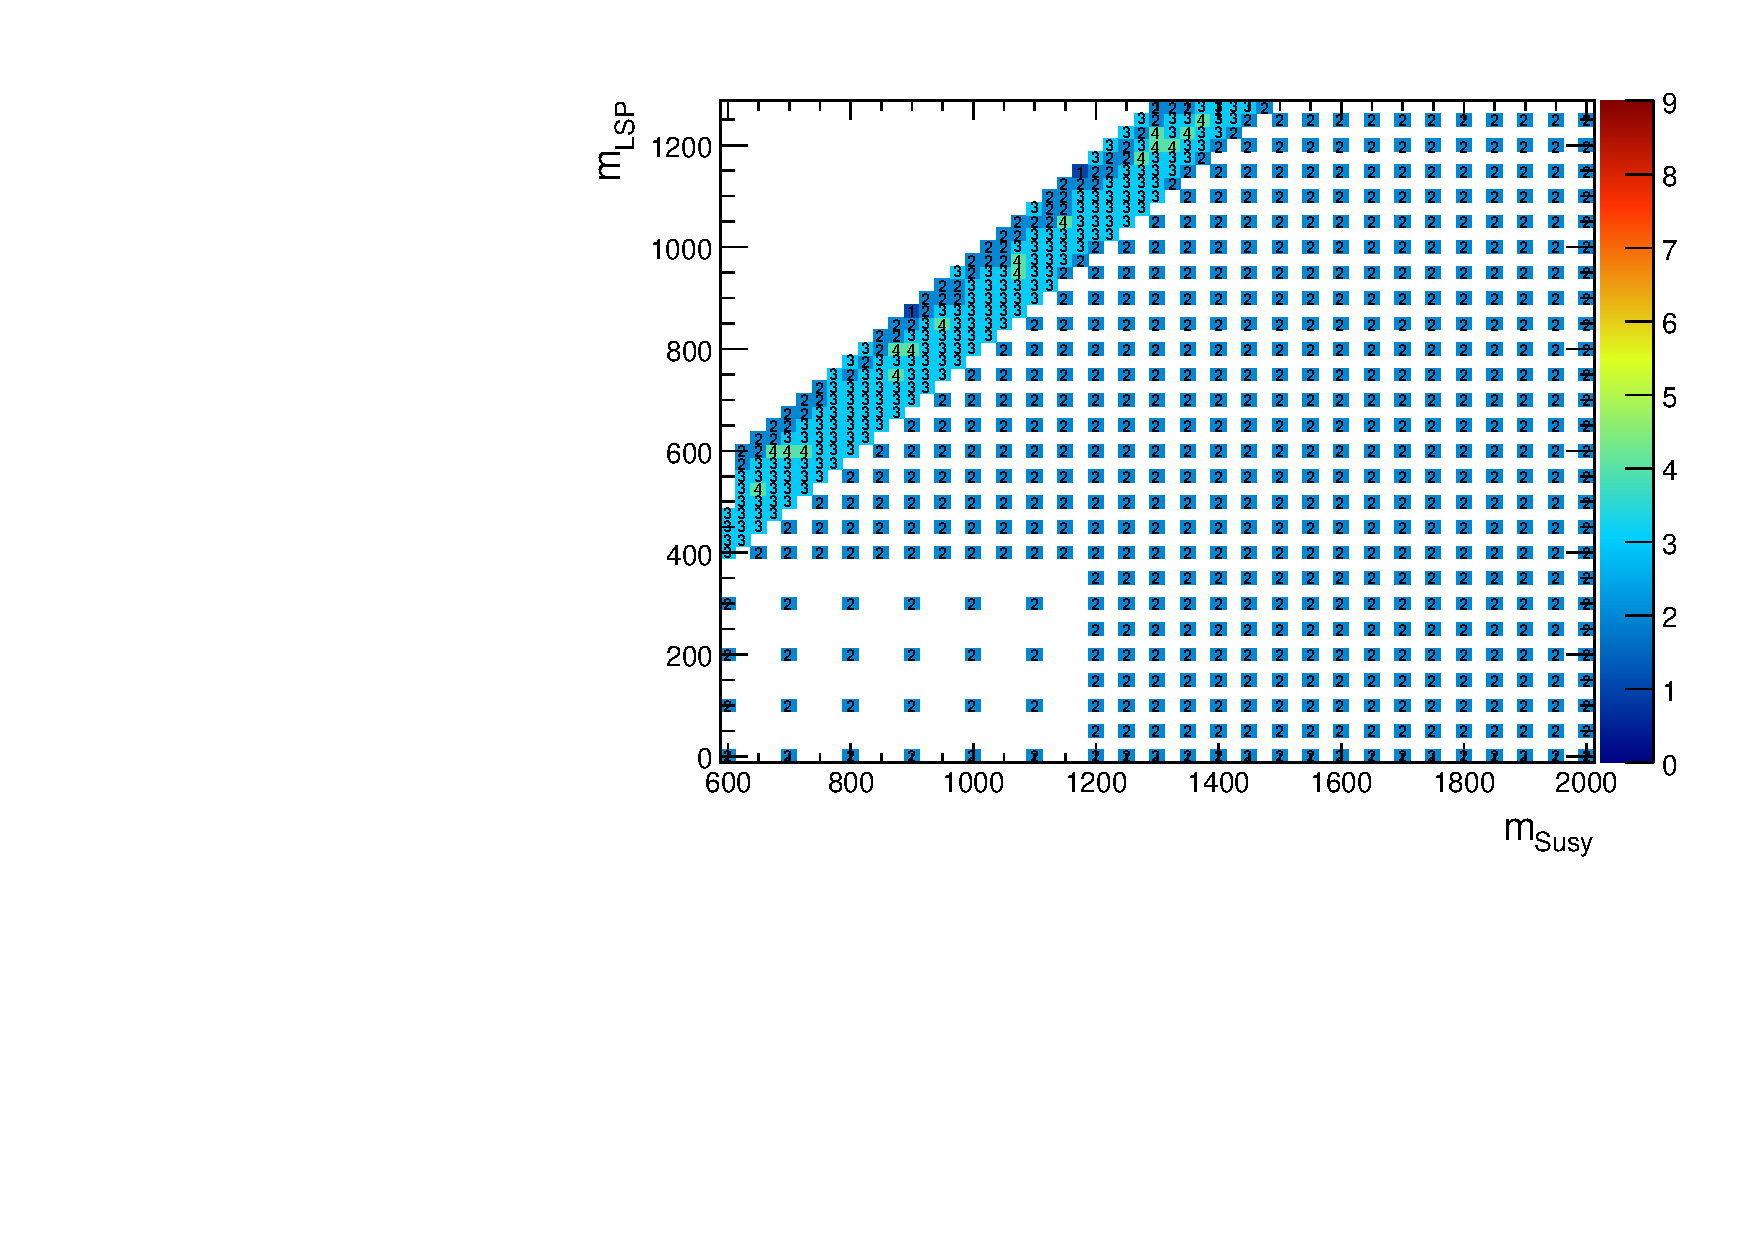
\includegraphics[width=0.33\textwidth]{figures/jetRanking/jetRankingT1qqqq_order2/T1qqqq_eq4j}} \\
    \subfigure[eq4a]{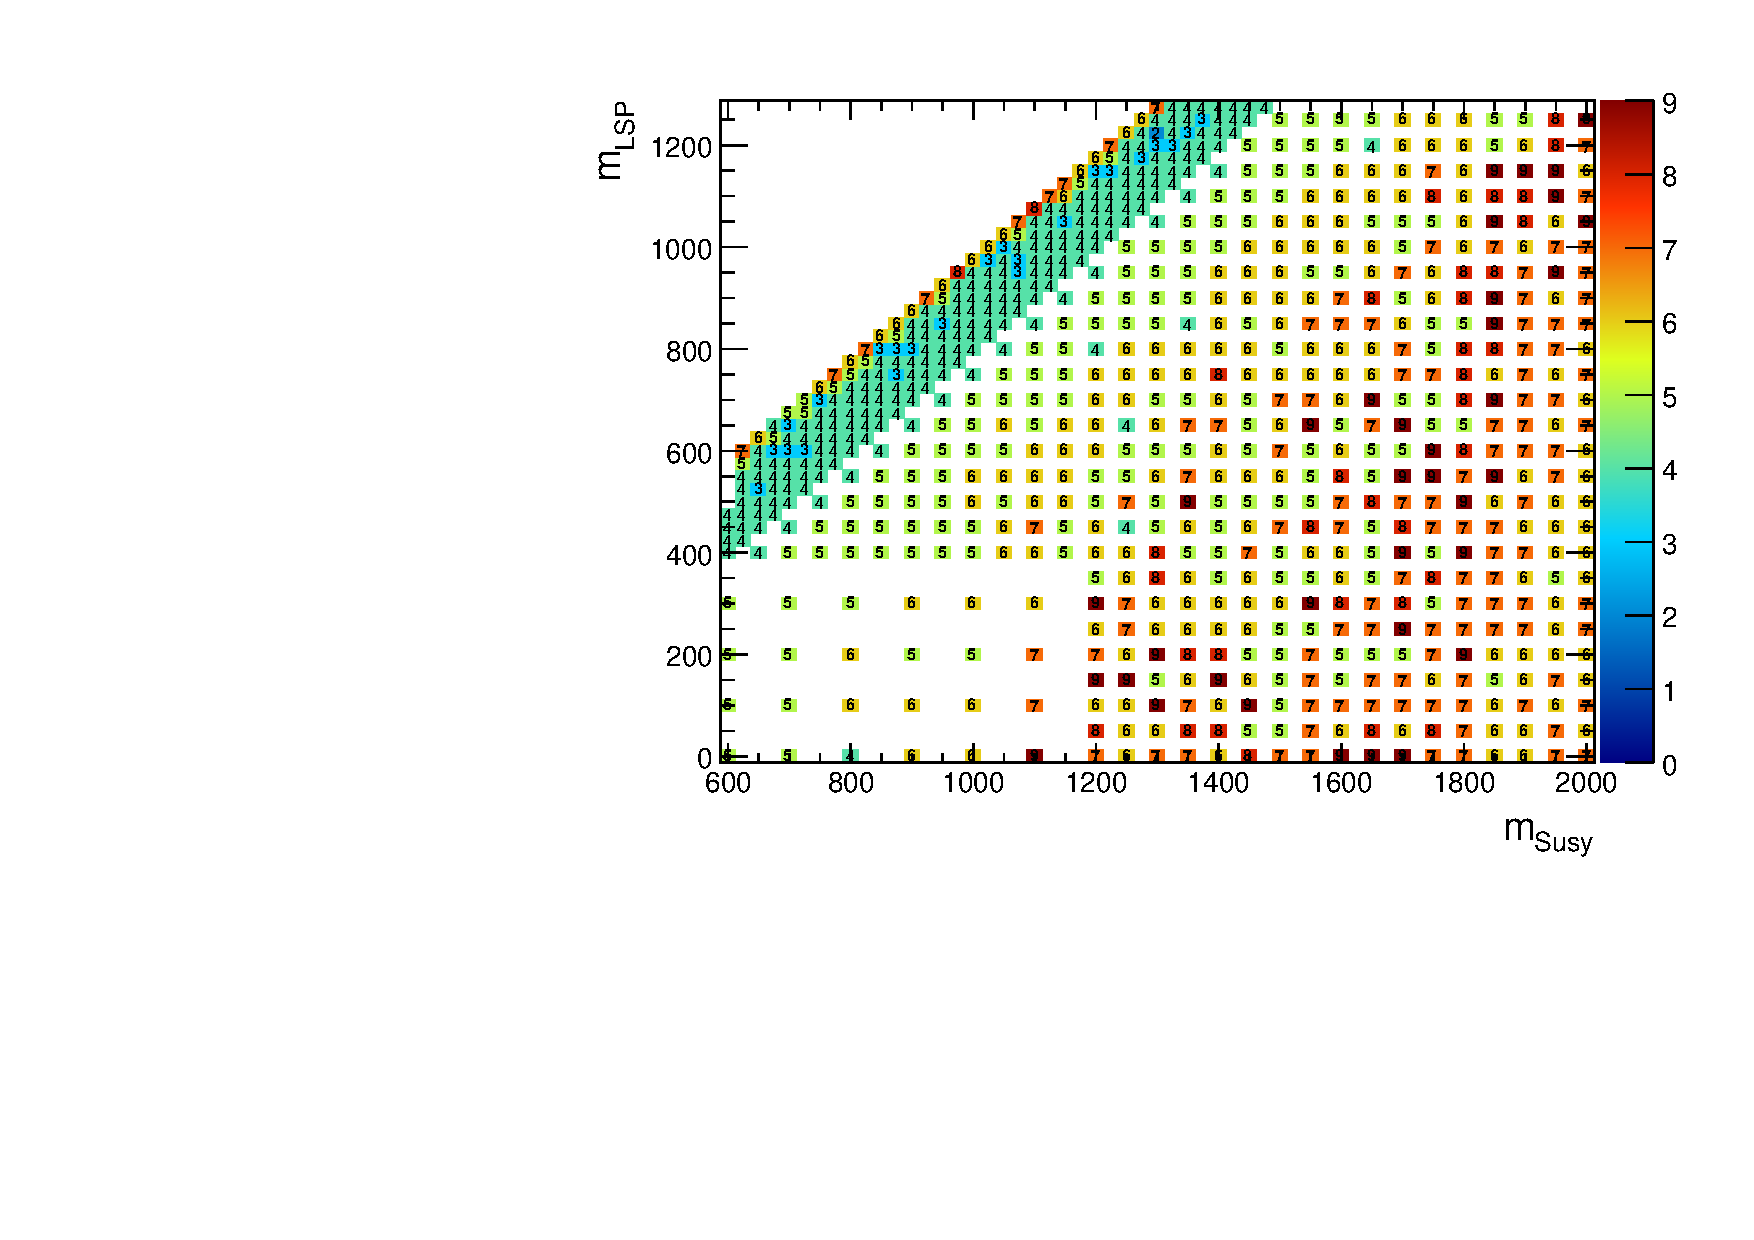
\includegraphics[width=0.33\textwidth]{figures/jetRanking/jetRankingT1qqqq_order2/T1qqqq_eq4a}} ~~
    \subfigure[eq3j]{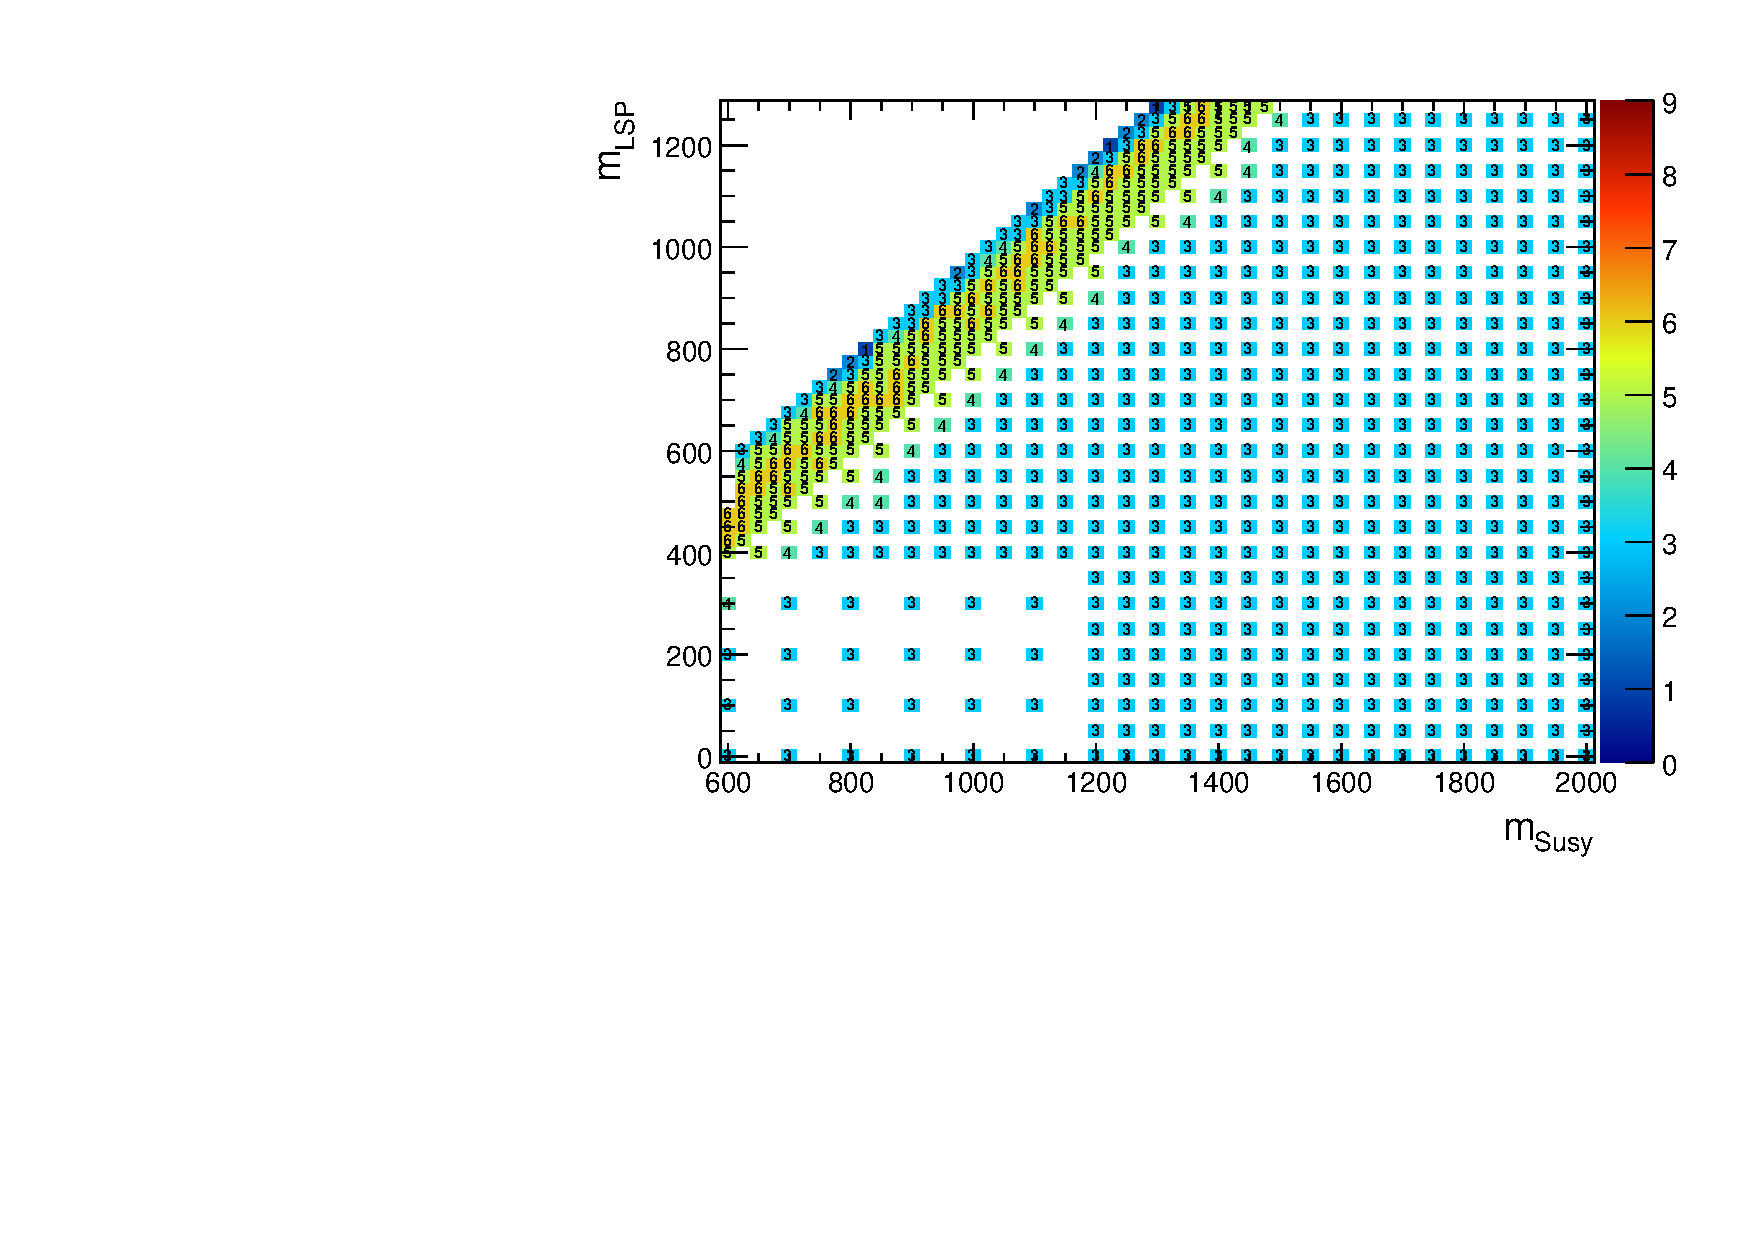
\includegraphics[width=0.33\textwidth]{figures/jetRanking/jetRankingT1qqqq_order2/T1qqqq_eq3j}} ~~
    \subfigure[eq3a]{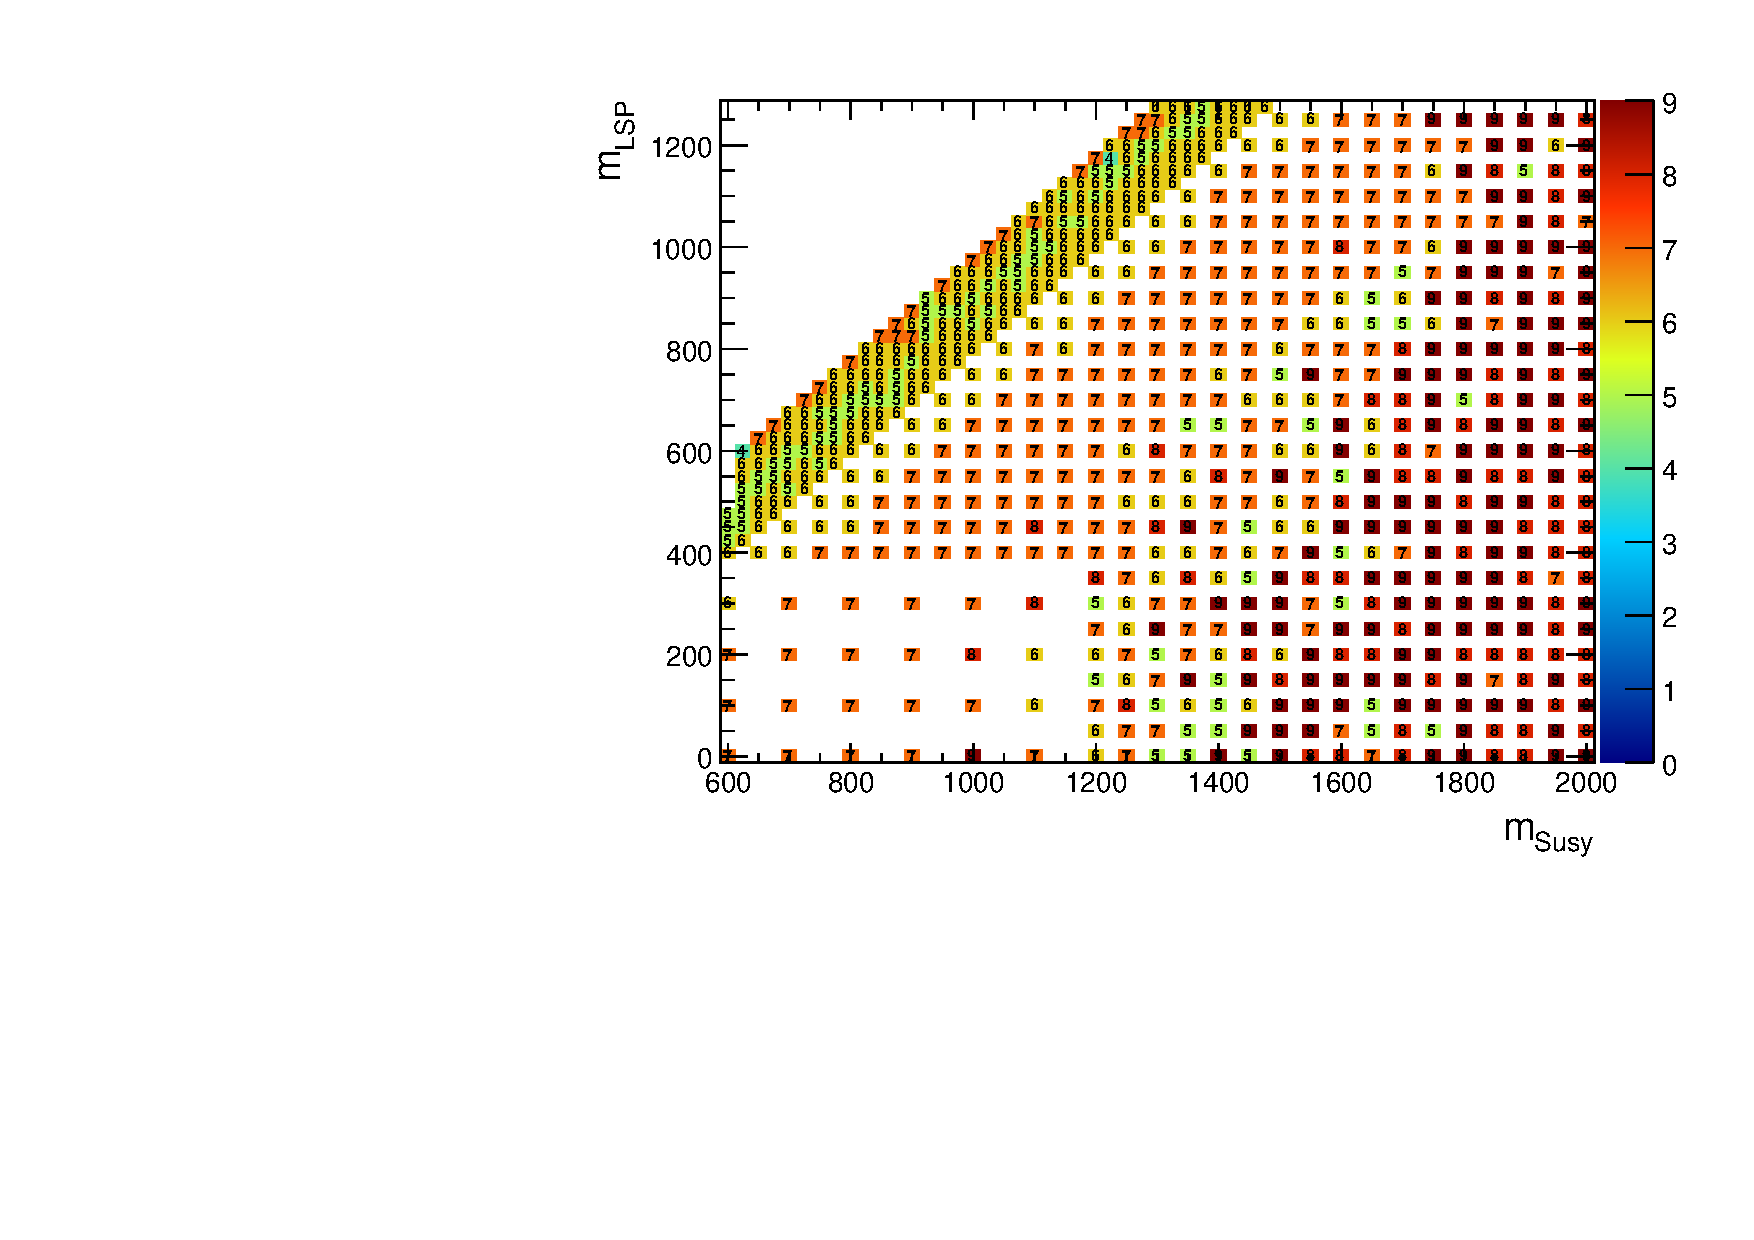
\includegraphics[width=0.33\textwidth]{figures/jetRanking/jetRankingT1qqqq_order2/T1qqqq_eq3a}} \\
    \subfigure[eq2j]{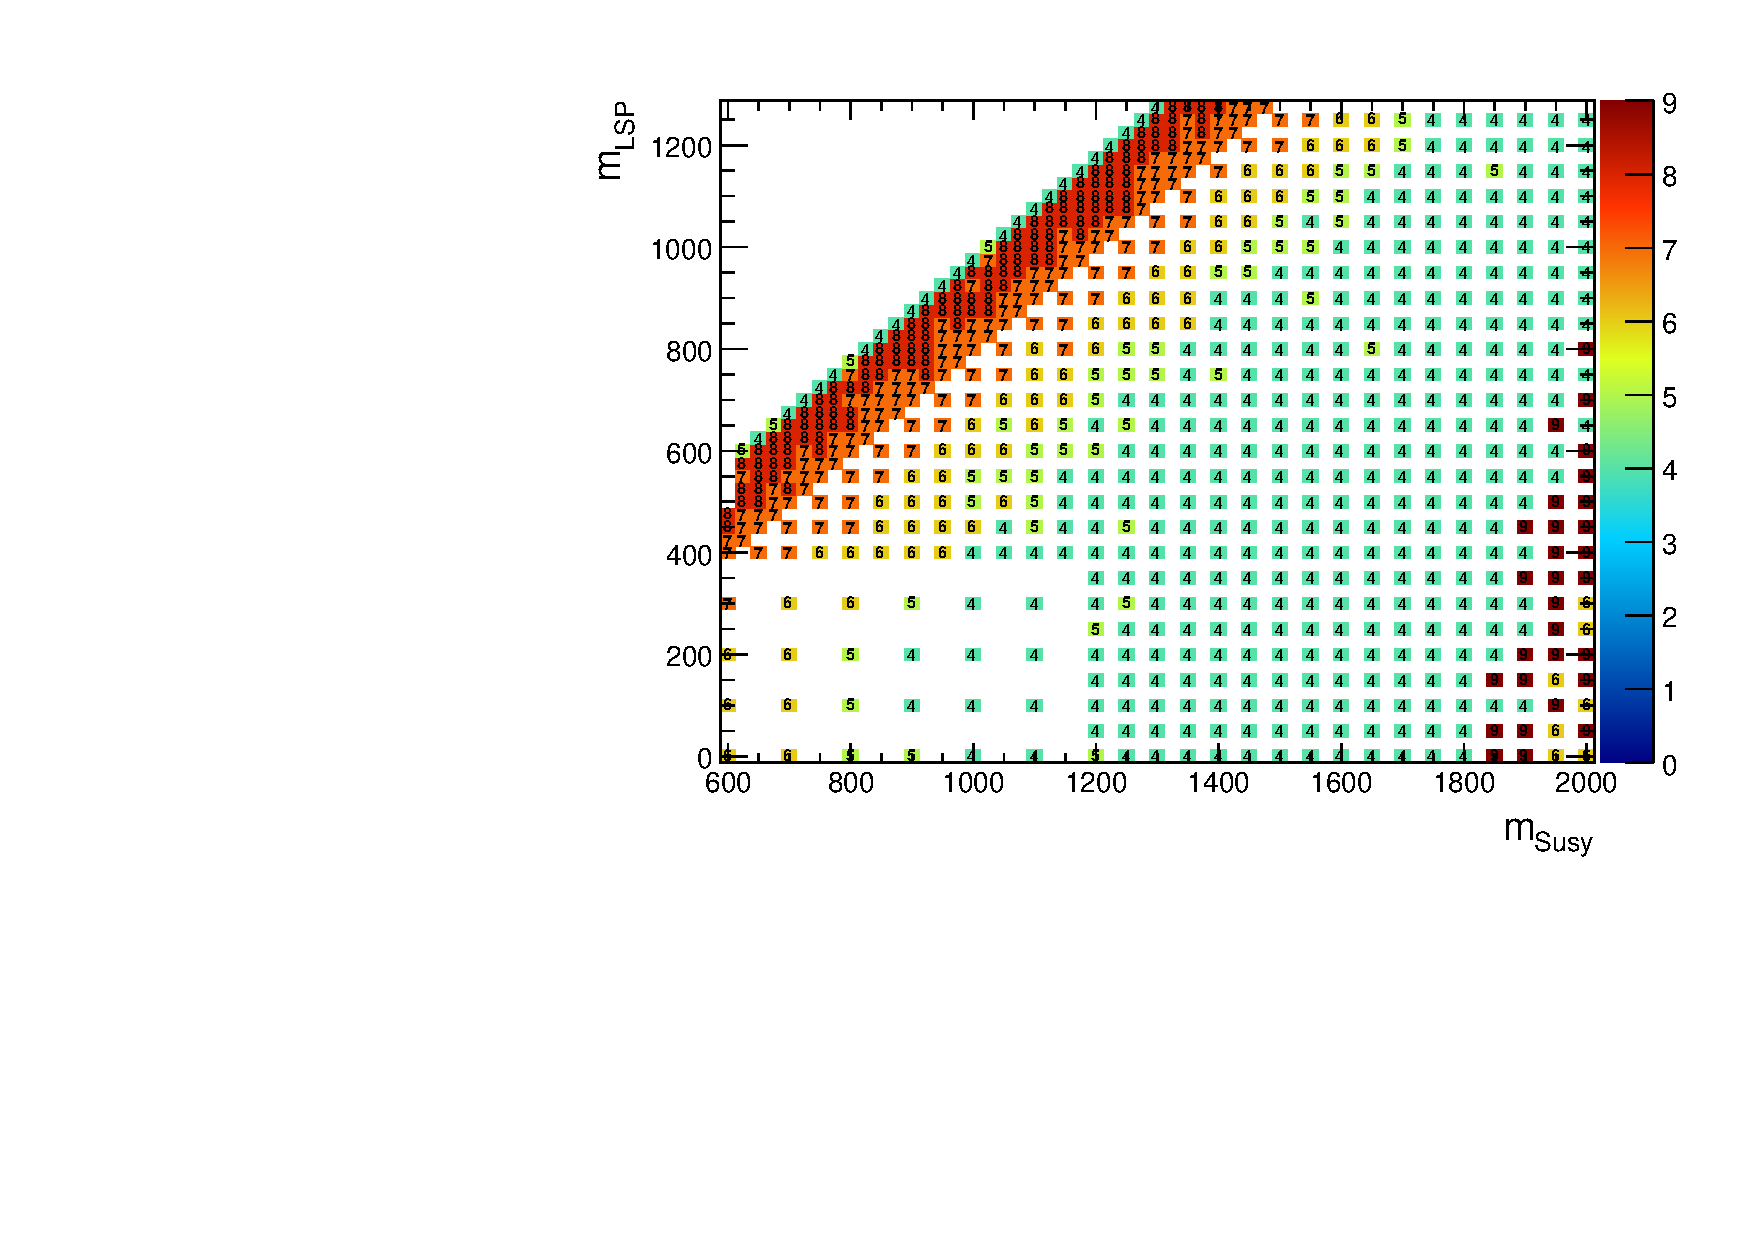
\includegraphics[width=0.33\textwidth]{figures/jetRanking/jetRankingT1qqqq_order2/T1qqqq_eq2j}} ~~
    \subfigure[eq2a]{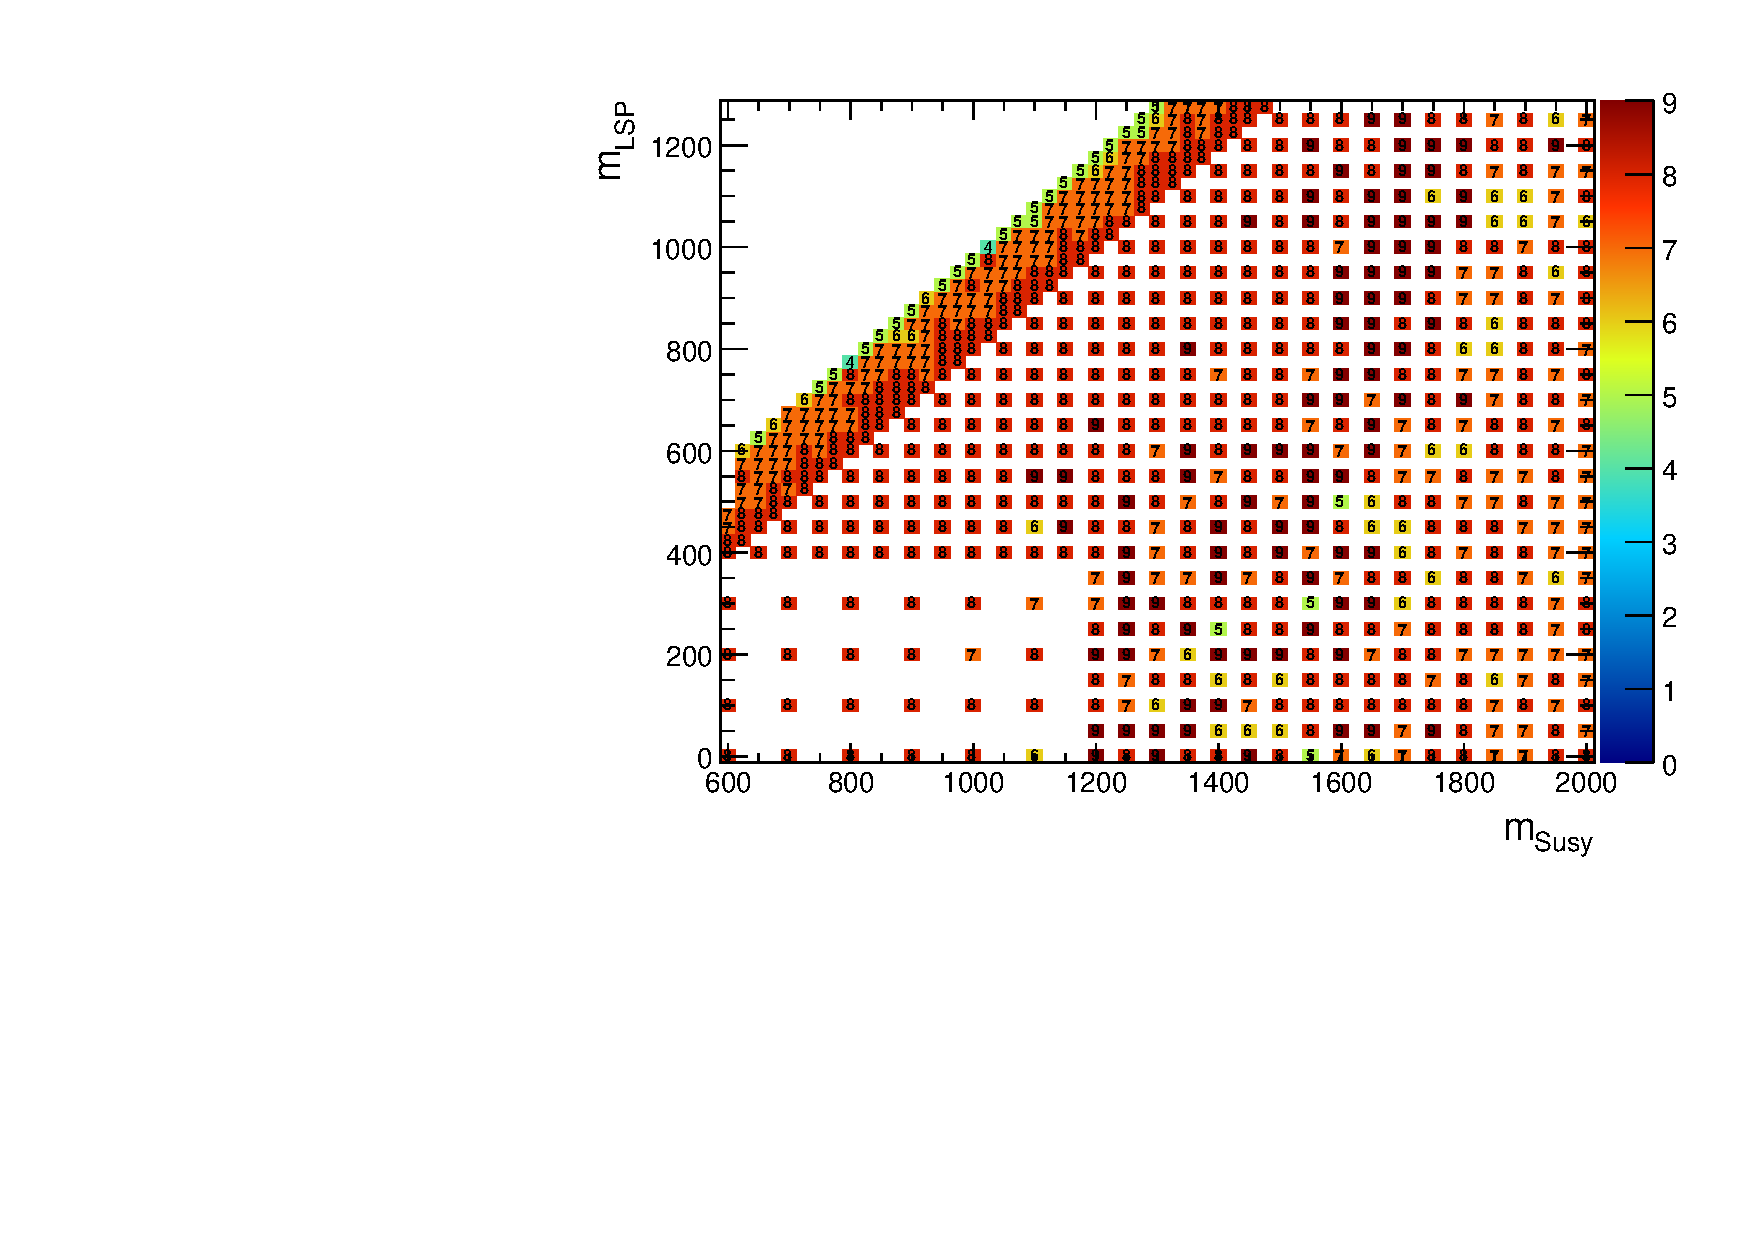
\includegraphics[width=0.33\textwidth]{figures/jetRanking/jetRankingT1qqqq_order2/T1qqqq_eq2a}} ~~
    \subfigure[eq1j]{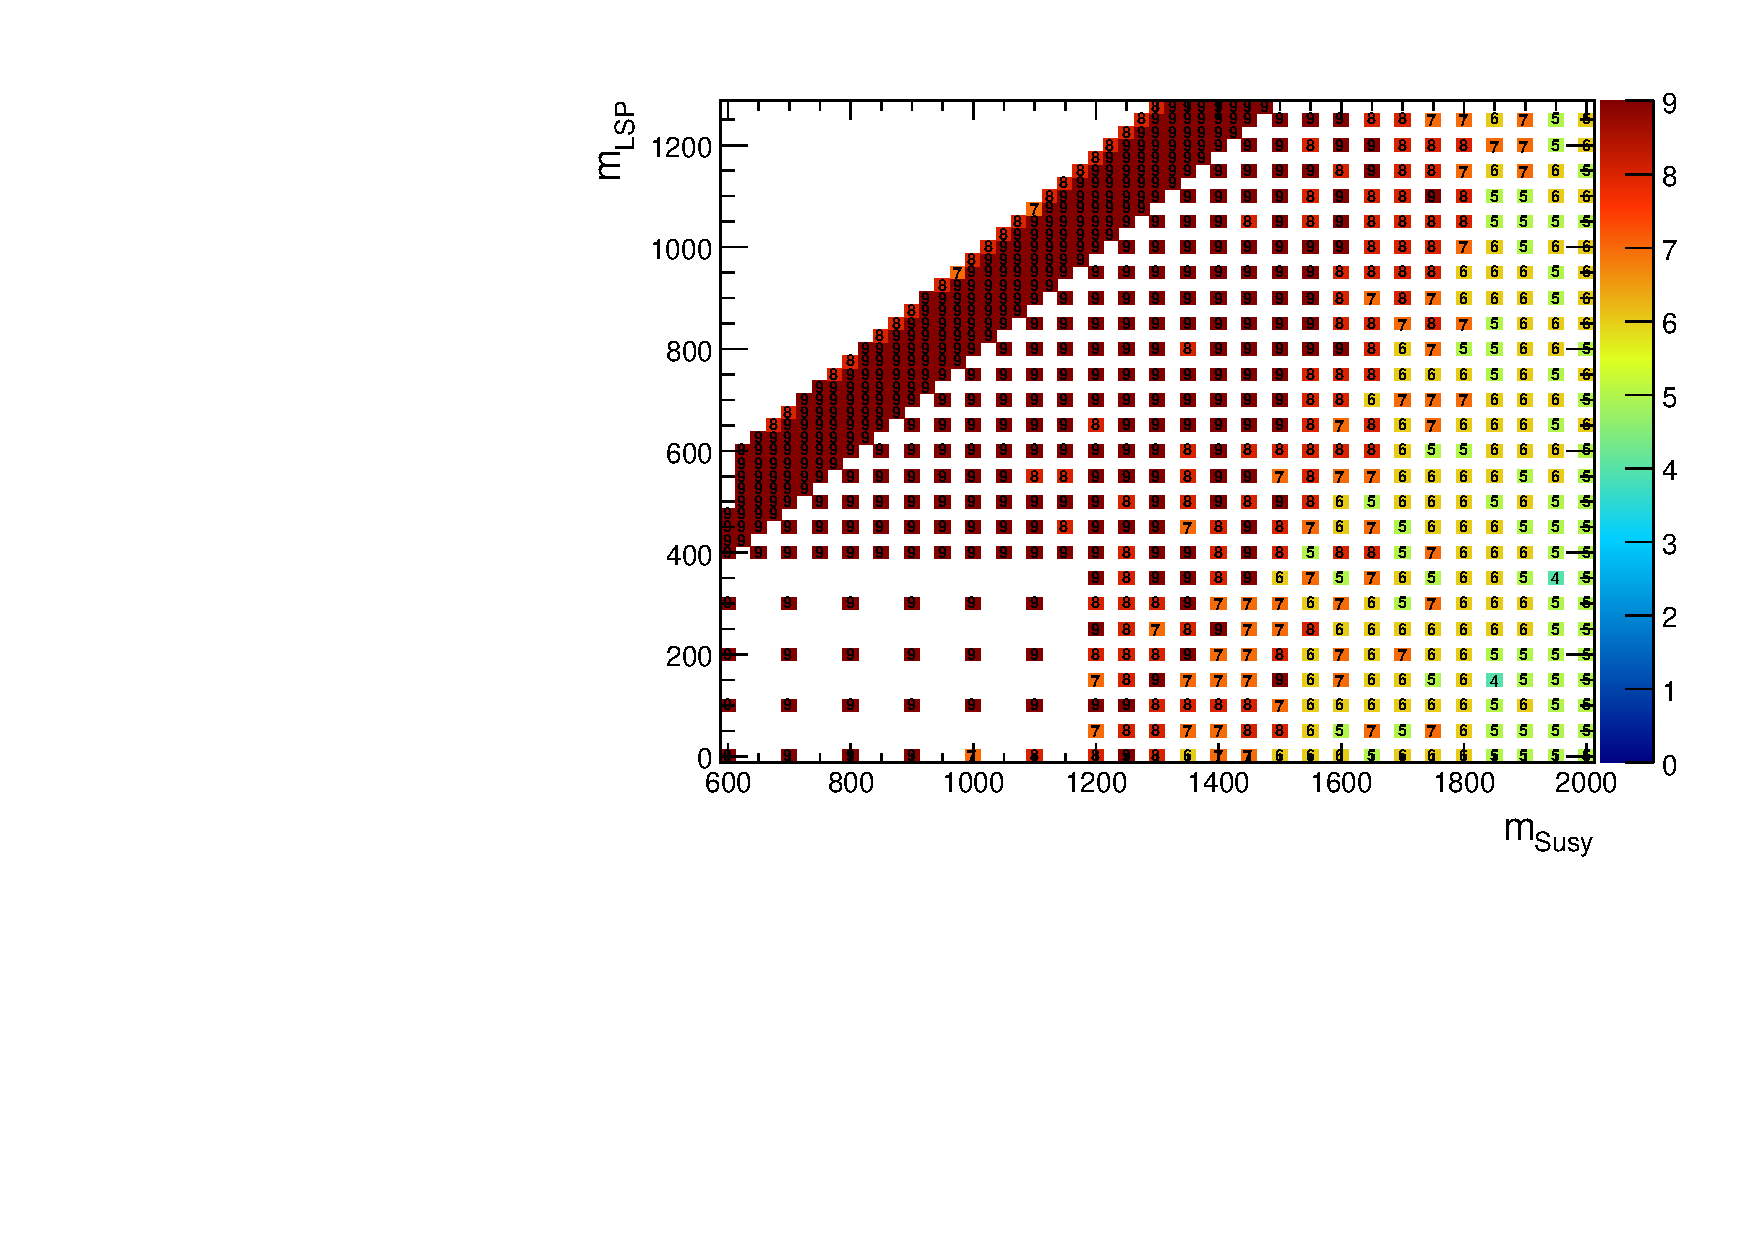
\includegraphics[width=0.33\textwidth]{figures/jetRanking/jetRankingT1qqqq_order2/T1qqqq_eq1j}} \\
  \end{center}
\end{figure}
\begin{figure}
  \caption{Ranking of each jet category across the mass plane for the T1tttt model
  \label{fig:rankingT1tttt}}
  \begin{center}    
    \subfigure[ge5j]{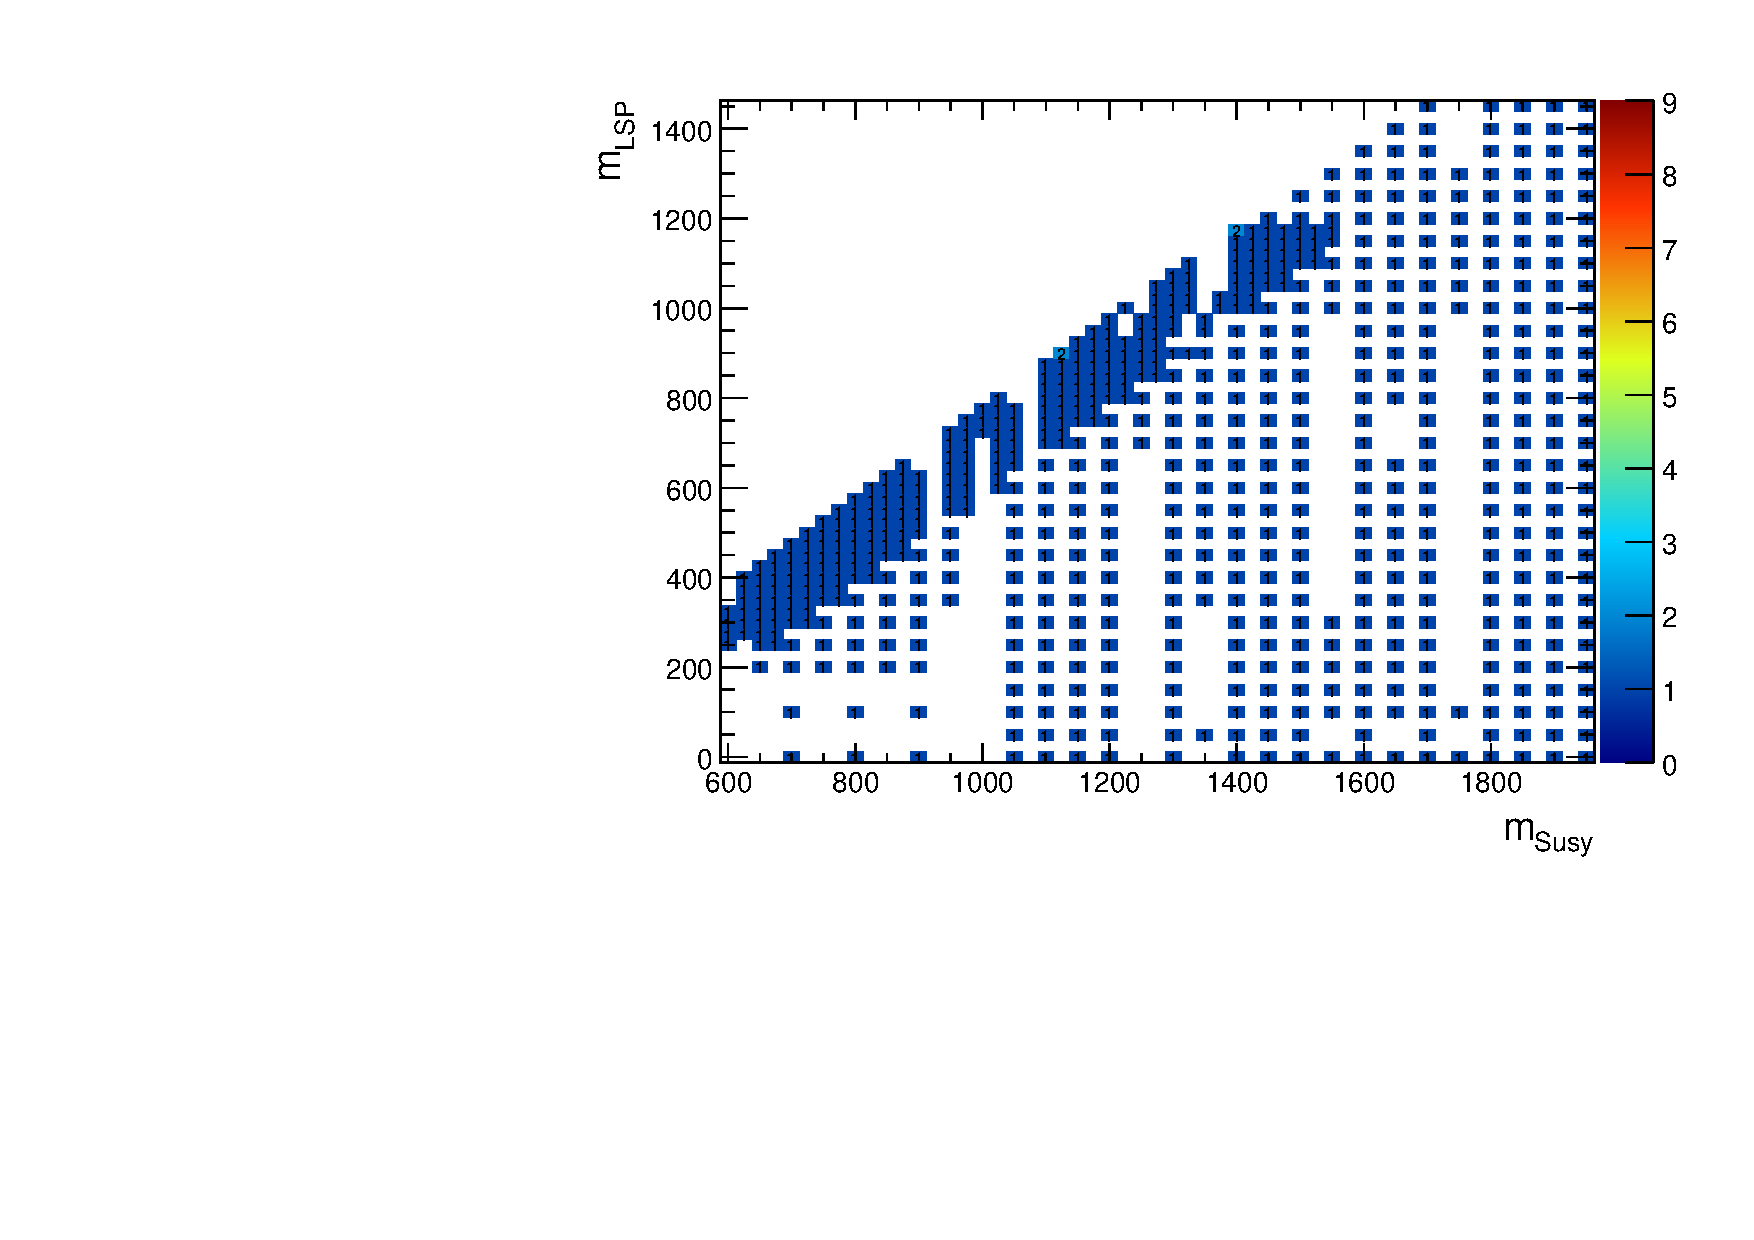
\includegraphics[width=0.33\textwidth]{figures/jetRanking/jetRankingT1tttt_order2/T1tttt_ge5j}} ~~
    \subfigure[ge5a]{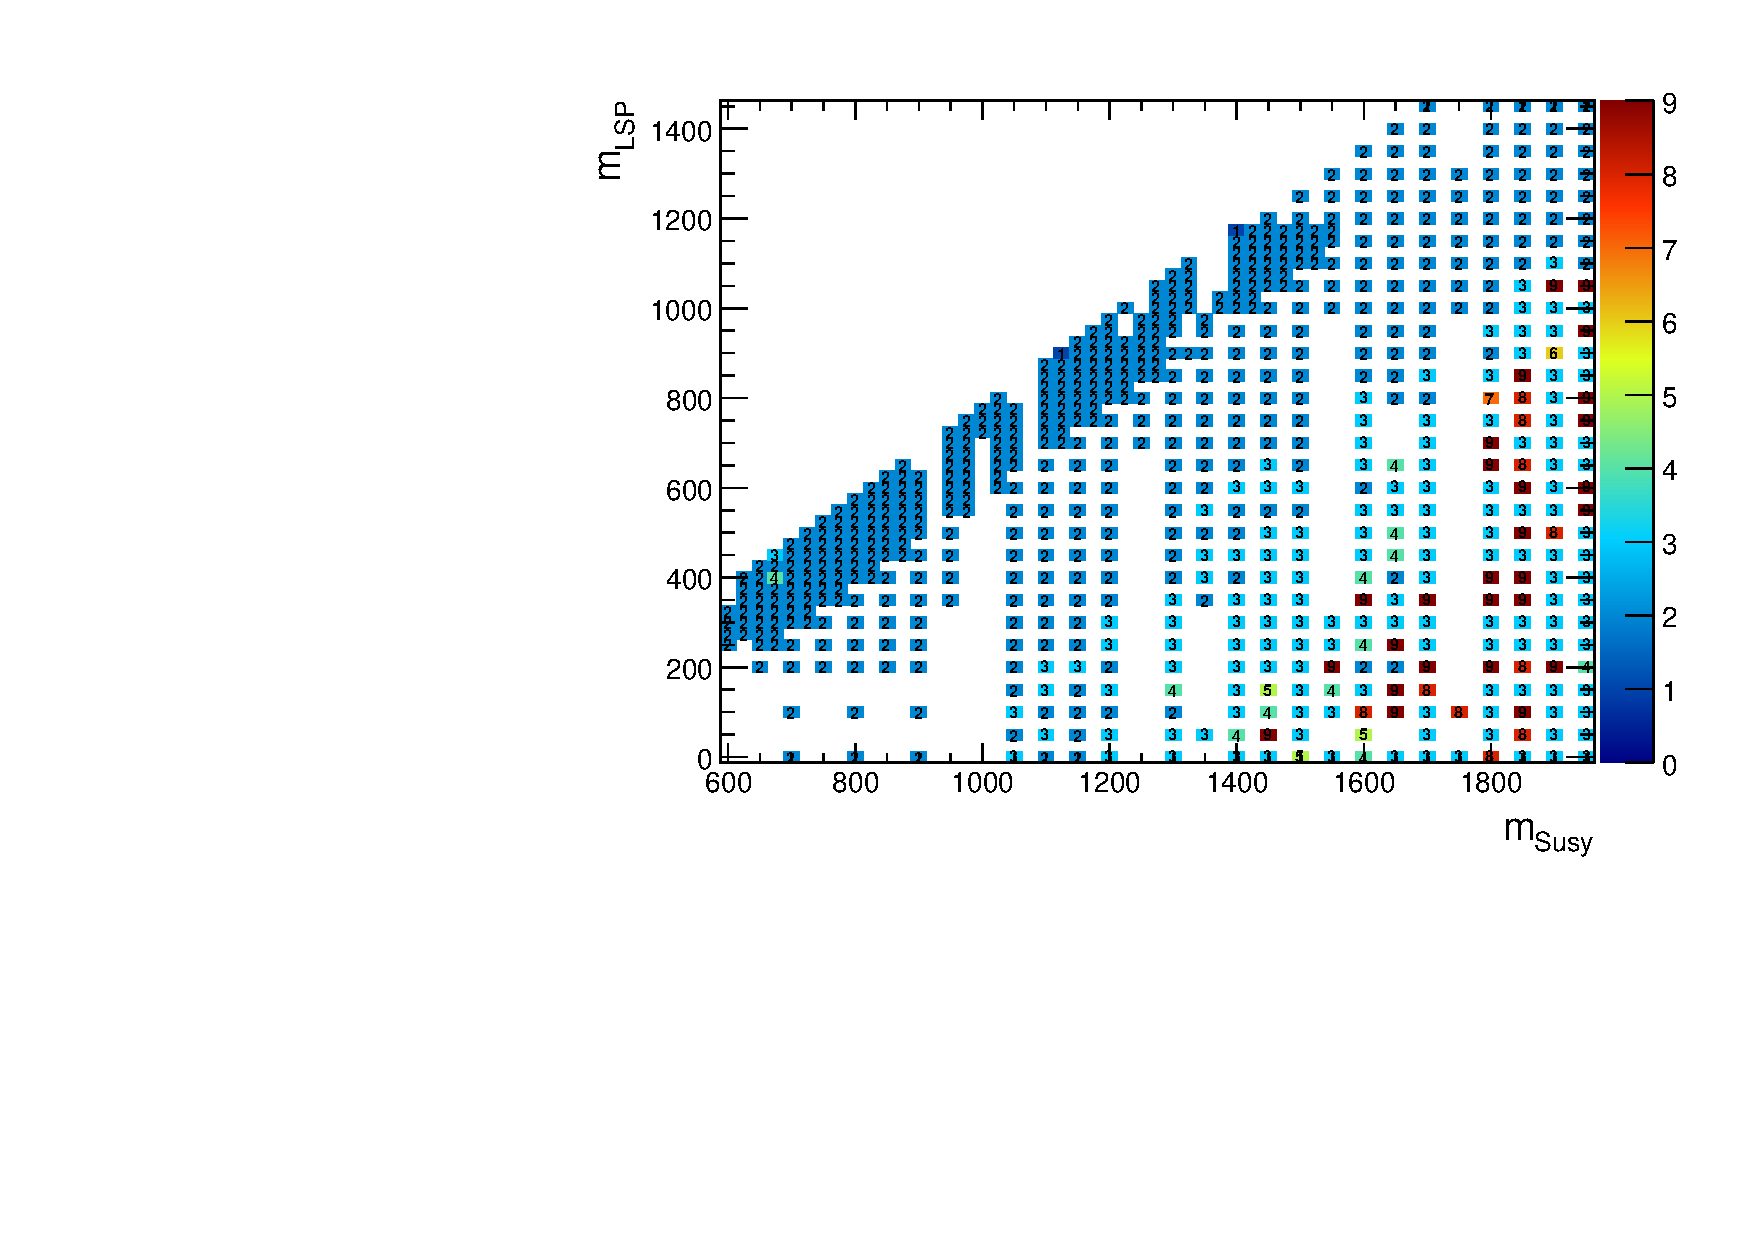
\includegraphics[width=0.33\textwidth]{figures/jetRanking/jetRankingT1tttt_order2/T1tttt_ge5a}} ~~
    \subfigure[eq4j]{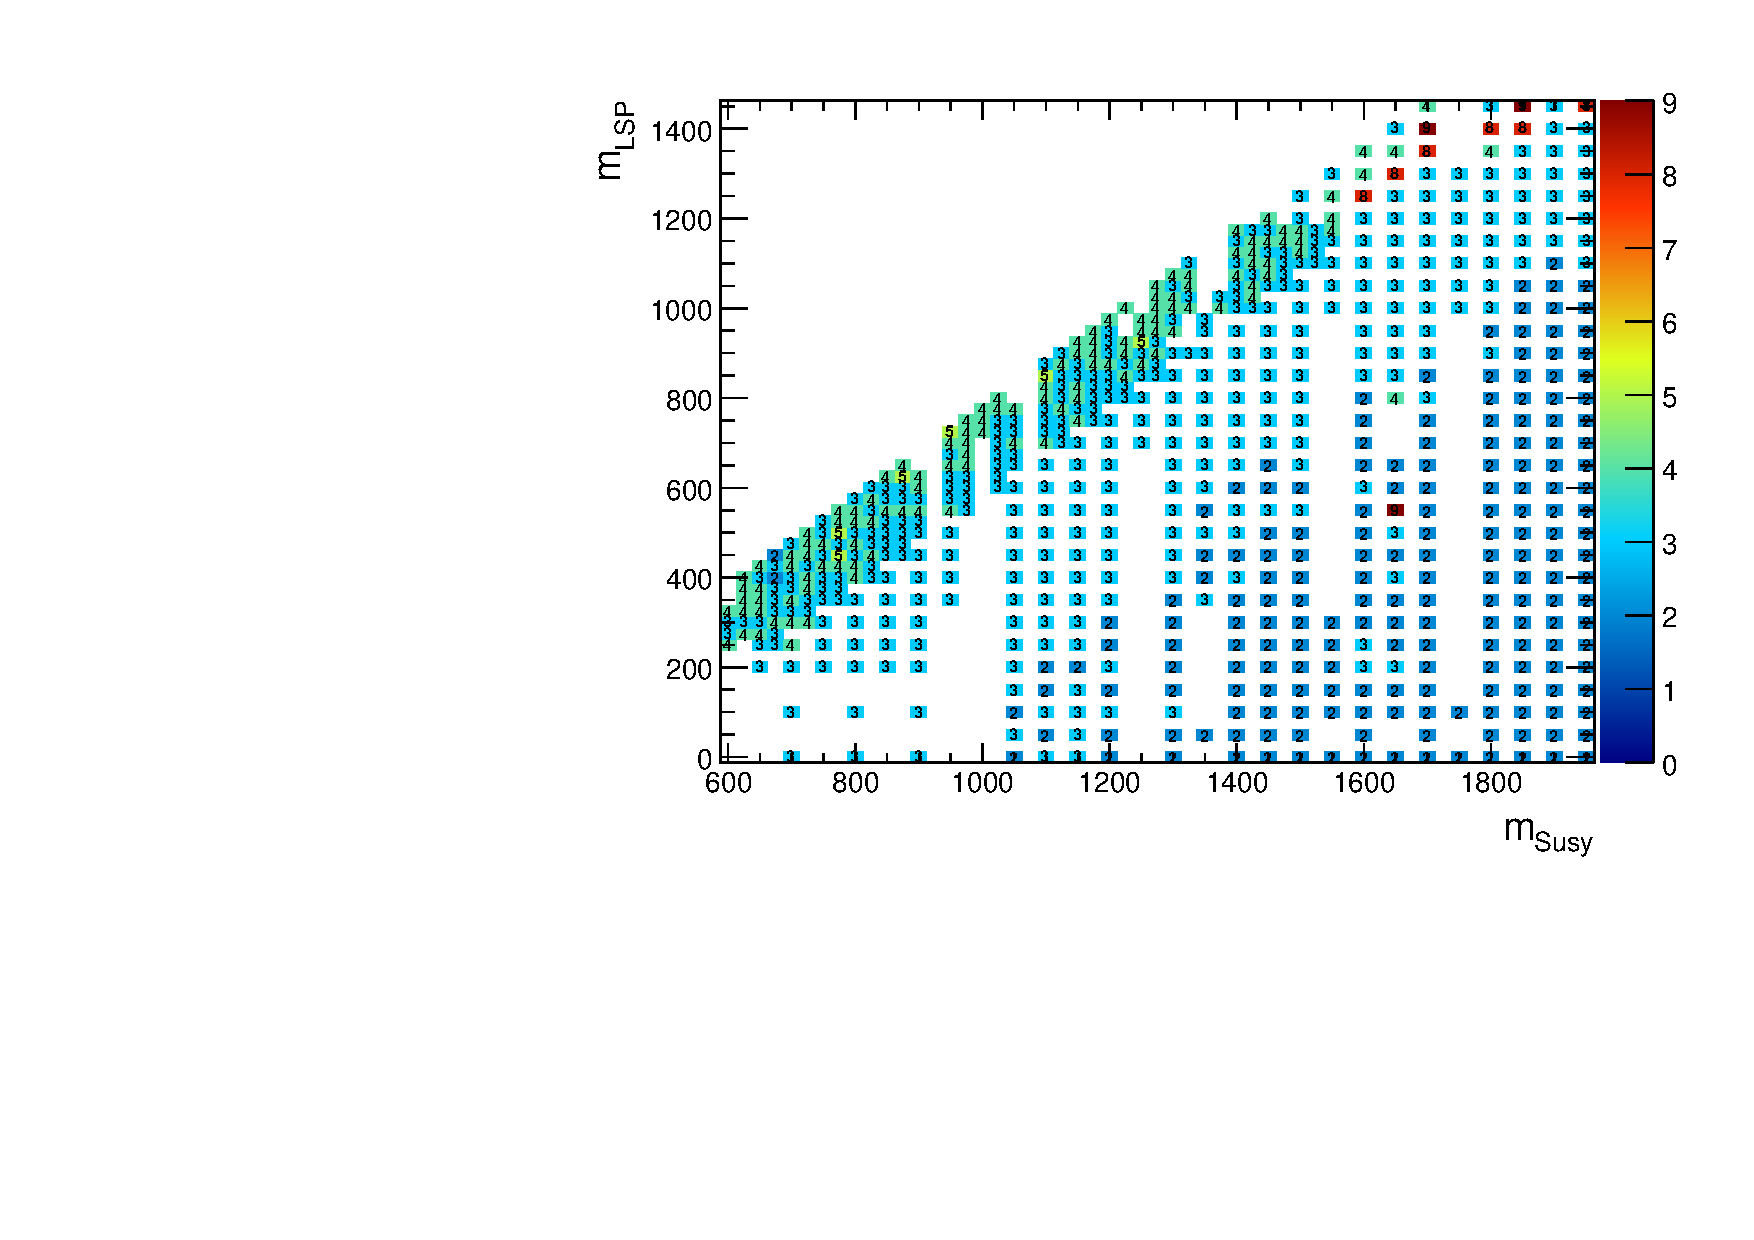
\includegraphics[width=0.33\textwidth]{figures/jetRanking/jetRankingT1tttt_order2/T1tttt_eq4j}} \\
    \subfigure[eq4a]{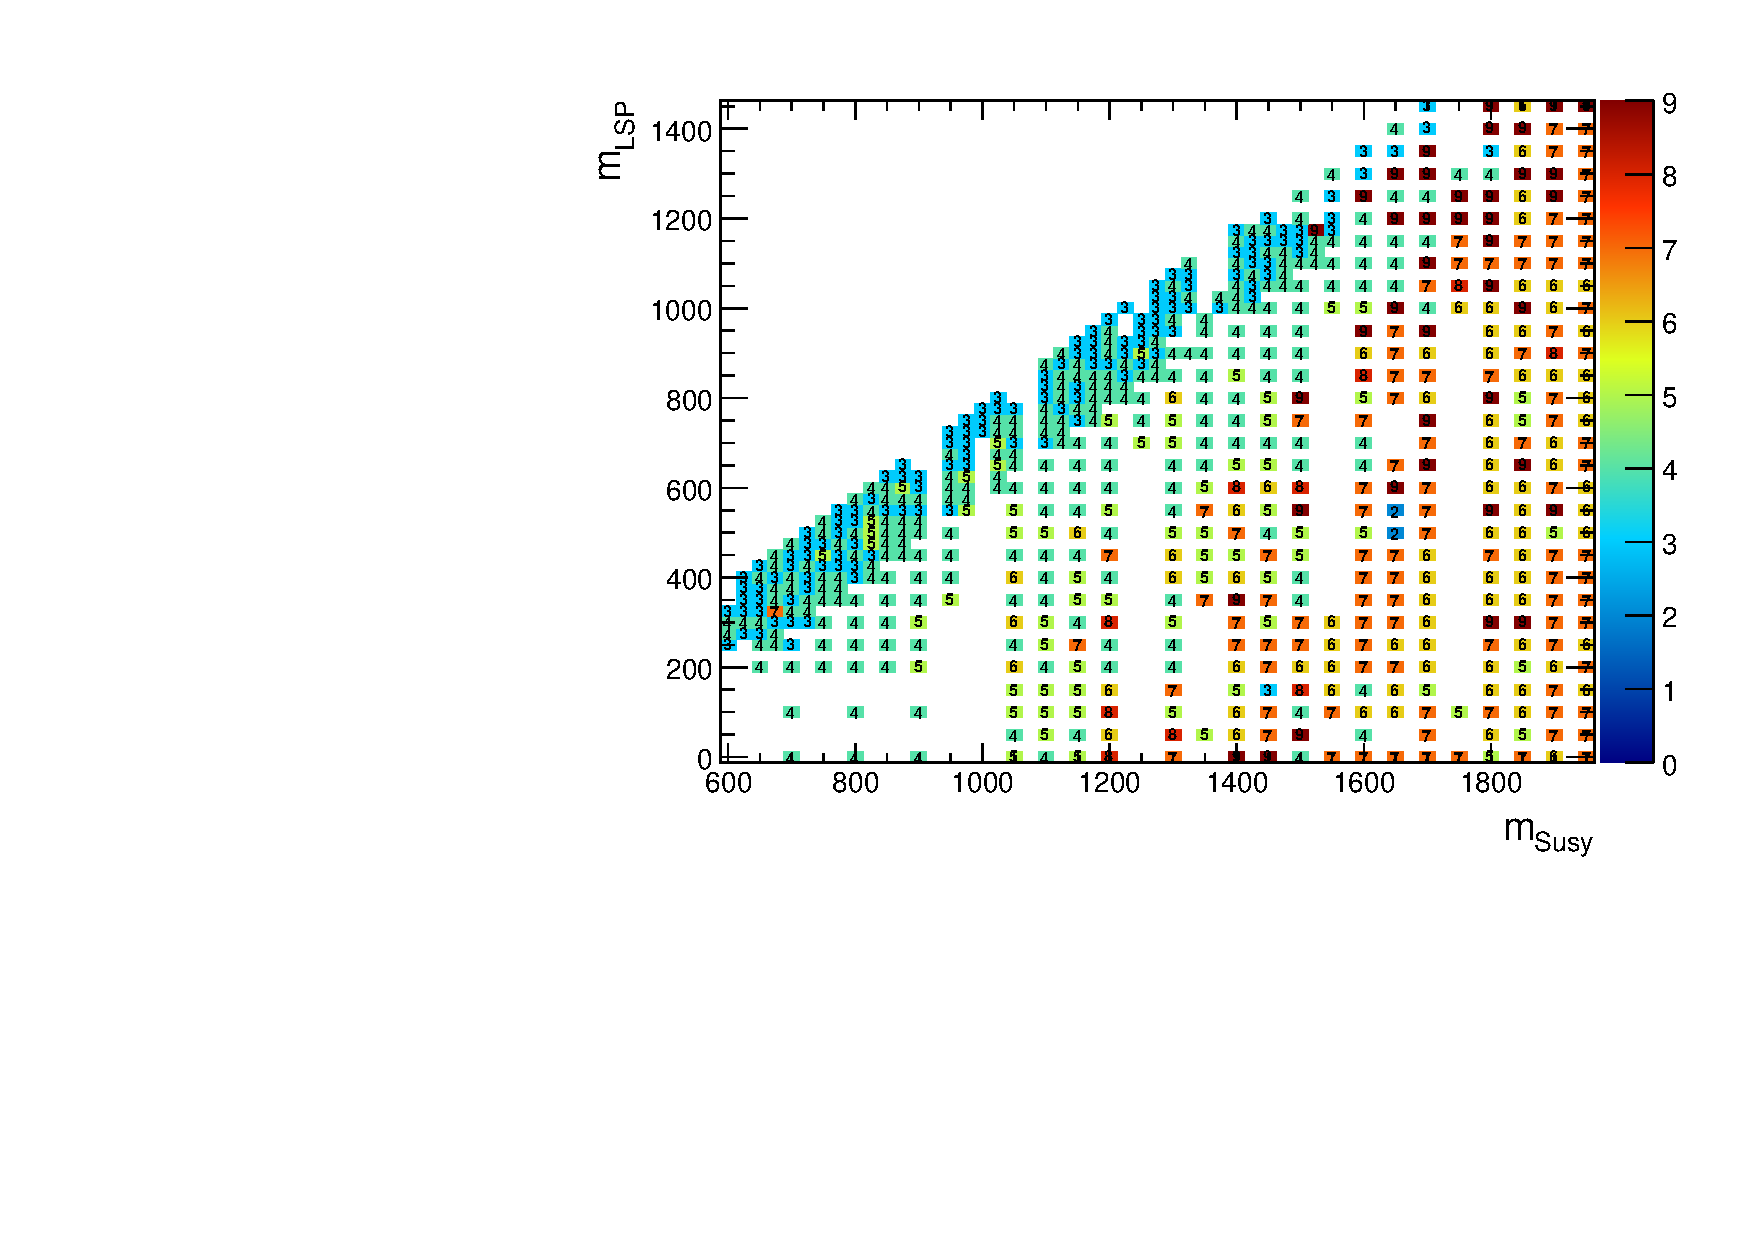
\includegraphics[width=0.33\textwidth]{figures/jetRanking/jetRankingT1tttt_order2/T1tttt_eq4a}} ~~
    \subfigure[eq3j]{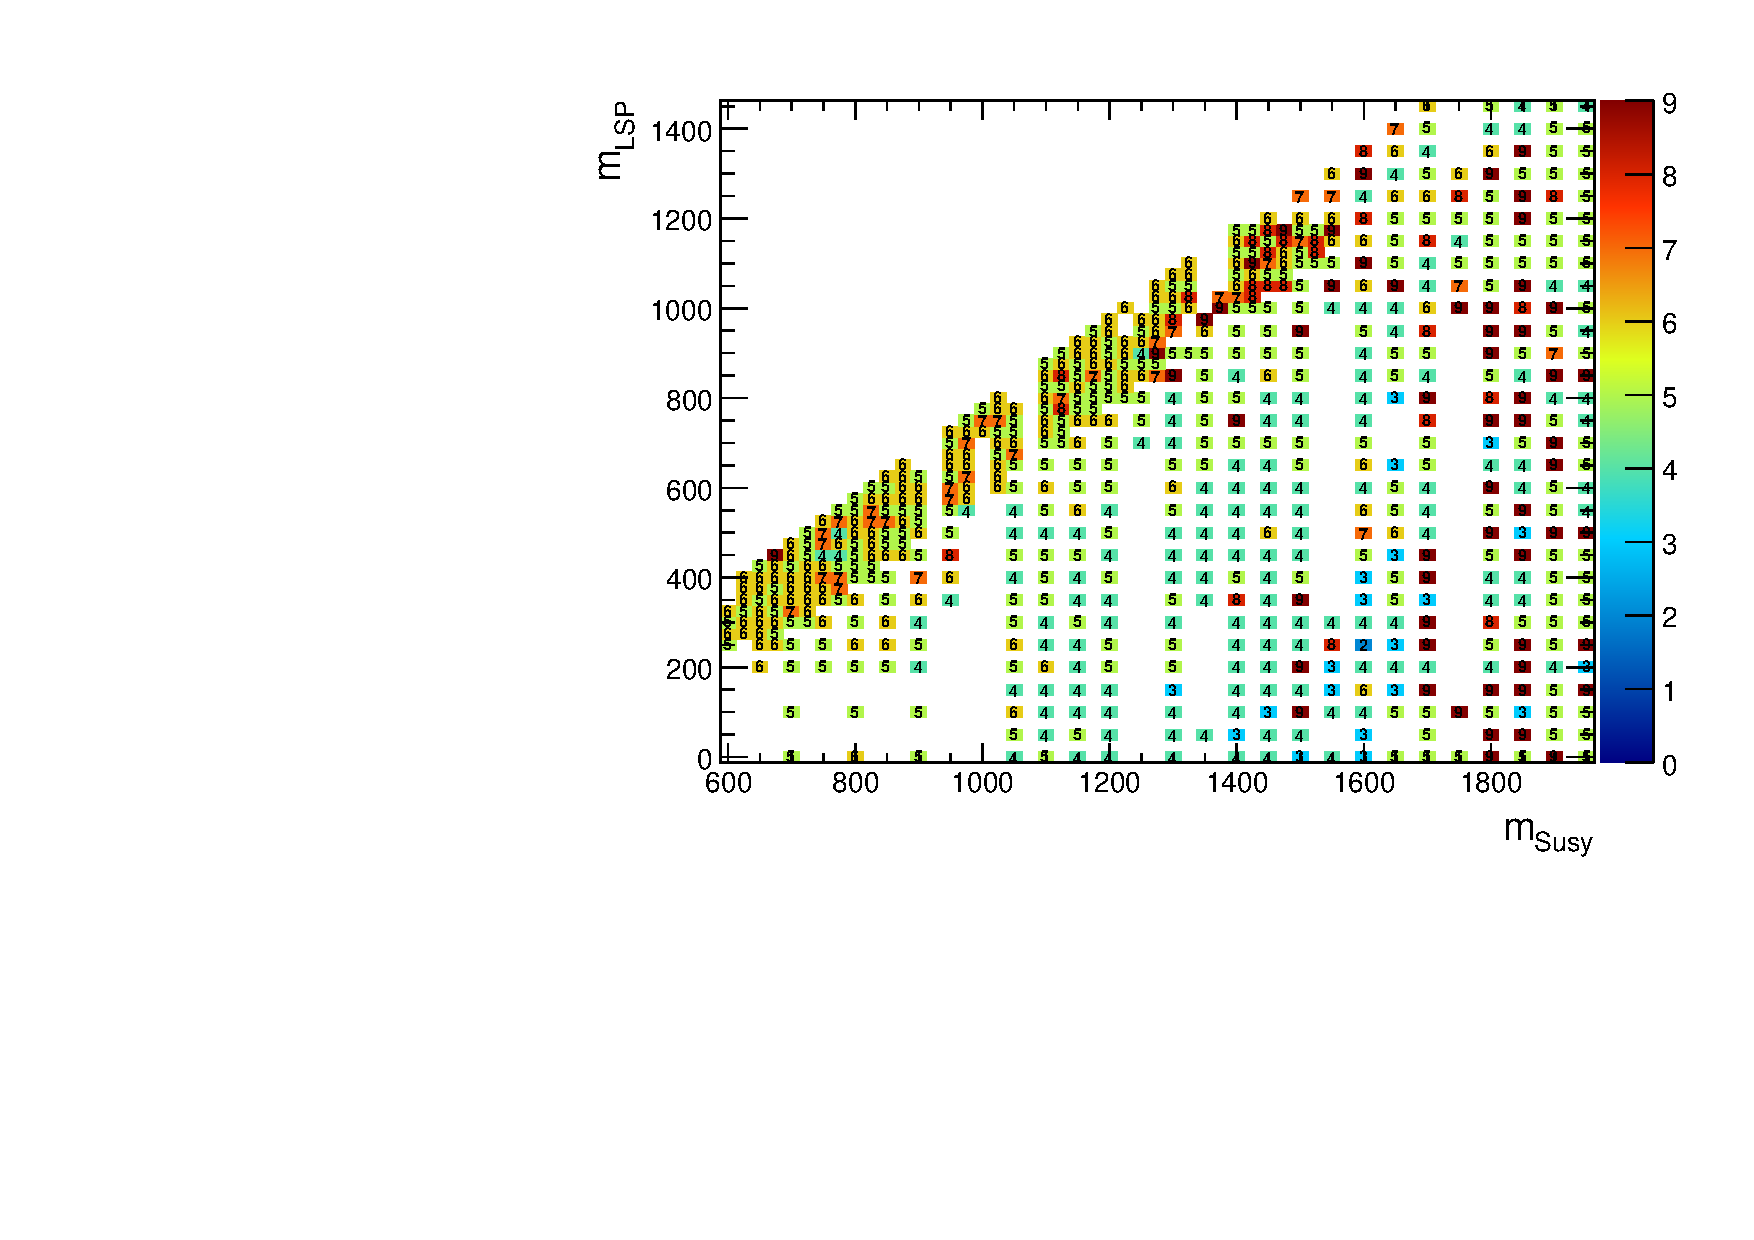
\includegraphics[width=0.33\textwidth]{figures/jetRanking/jetRankingT1tttt_order2/T1tttt_eq3j}} ~~
    \subfigure[eq3a]{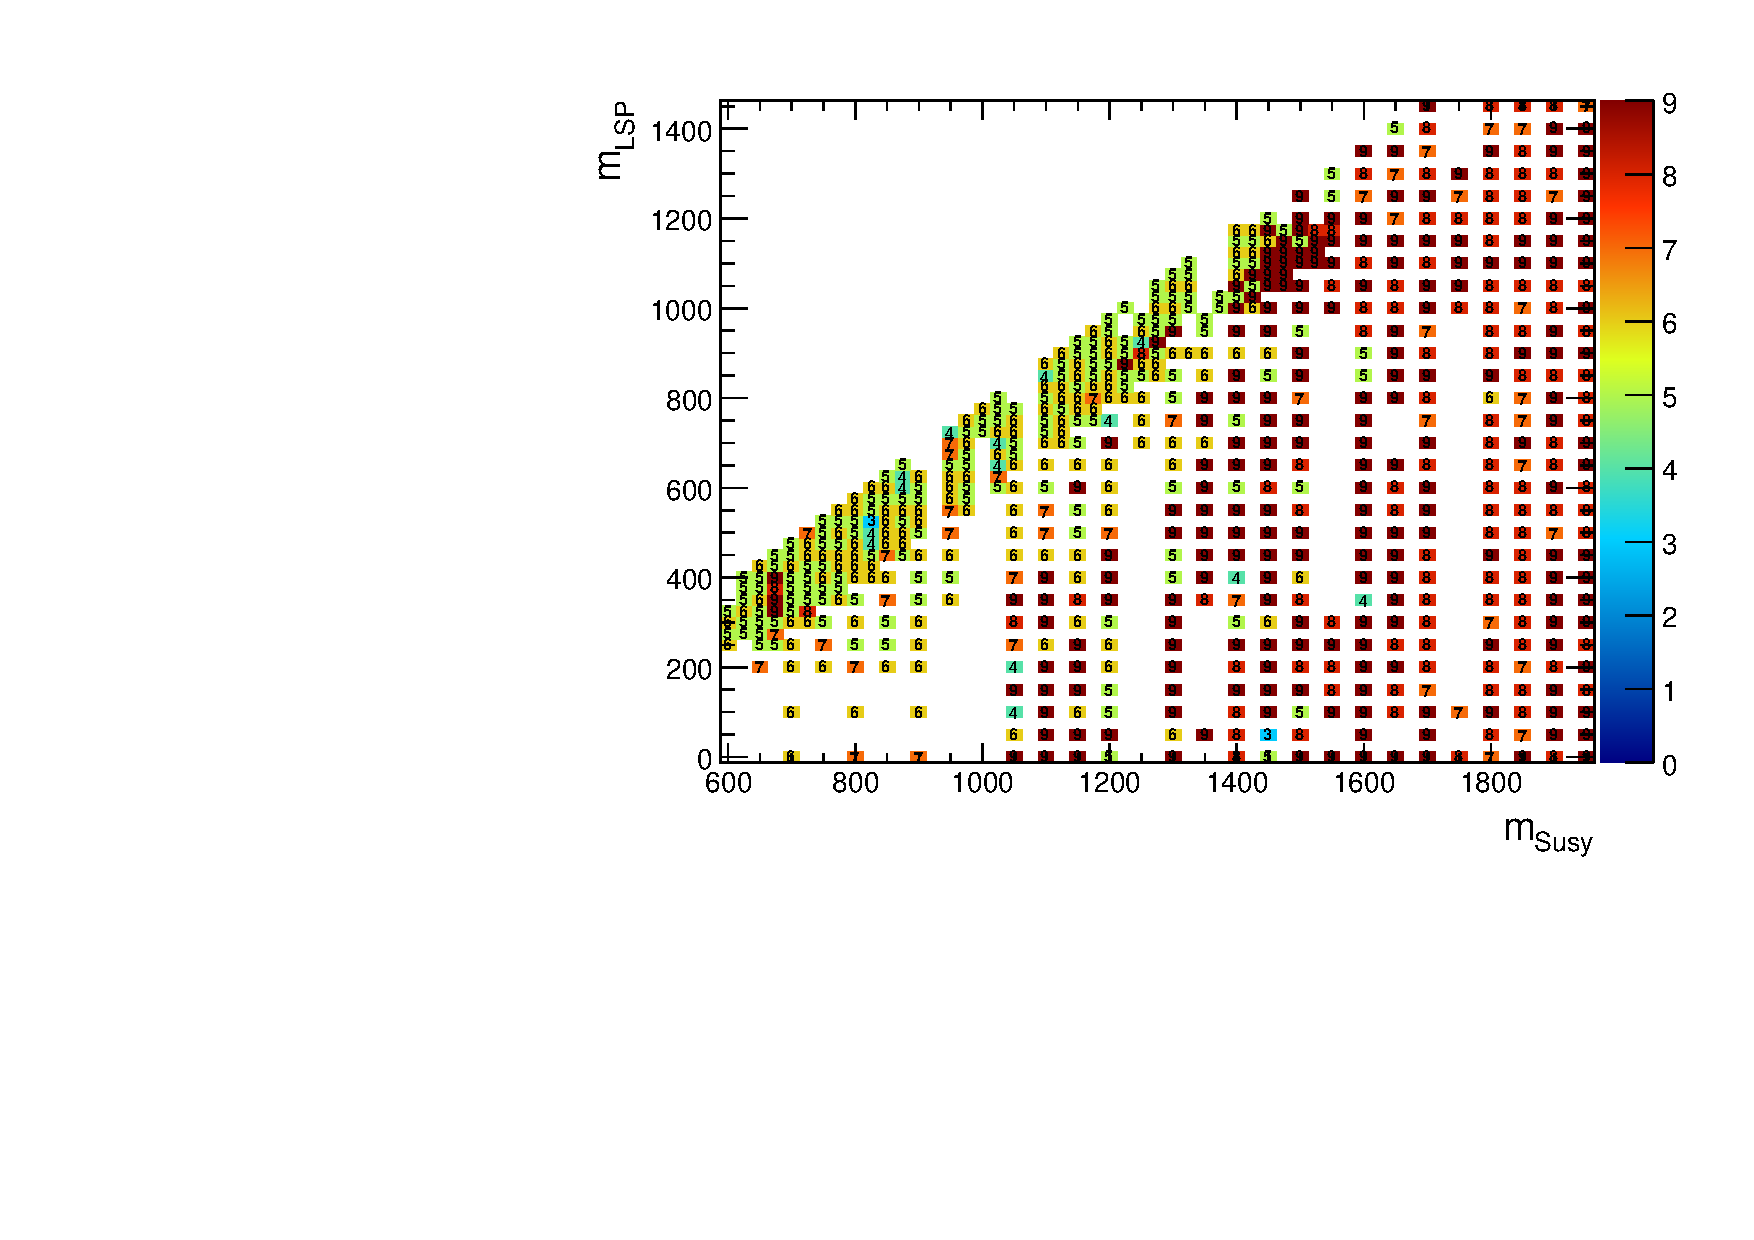
\includegraphics[width=0.33\textwidth]{figures/jetRanking/jetRankingT1tttt_order2/T1tttt_eq3a}} \\
    \subfigure[eq2j]{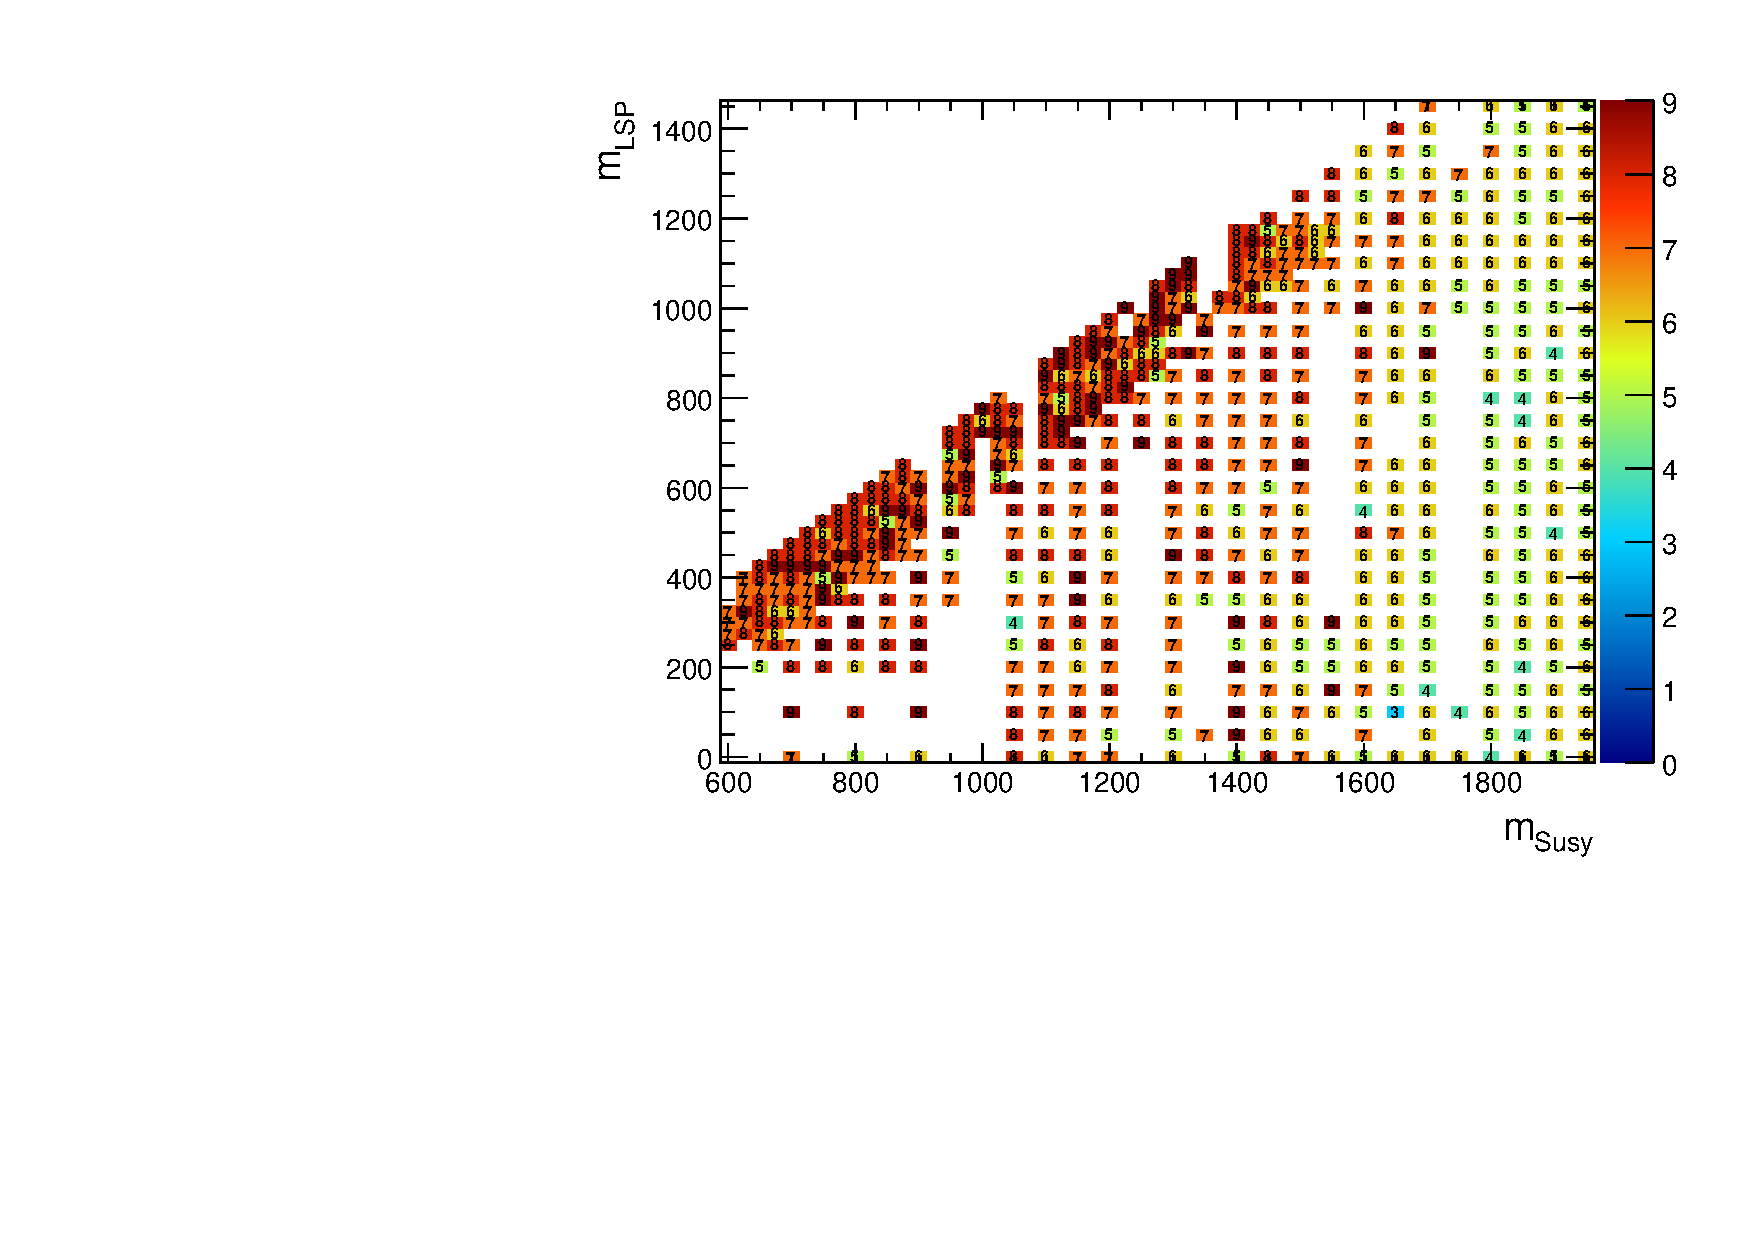
\includegraphics[width=0.33\textwidth]{figures/jetRanking/jetRankingT1tttt_order2/T1tttt_eq2j}} ~~
    \subfigure[eq2a]{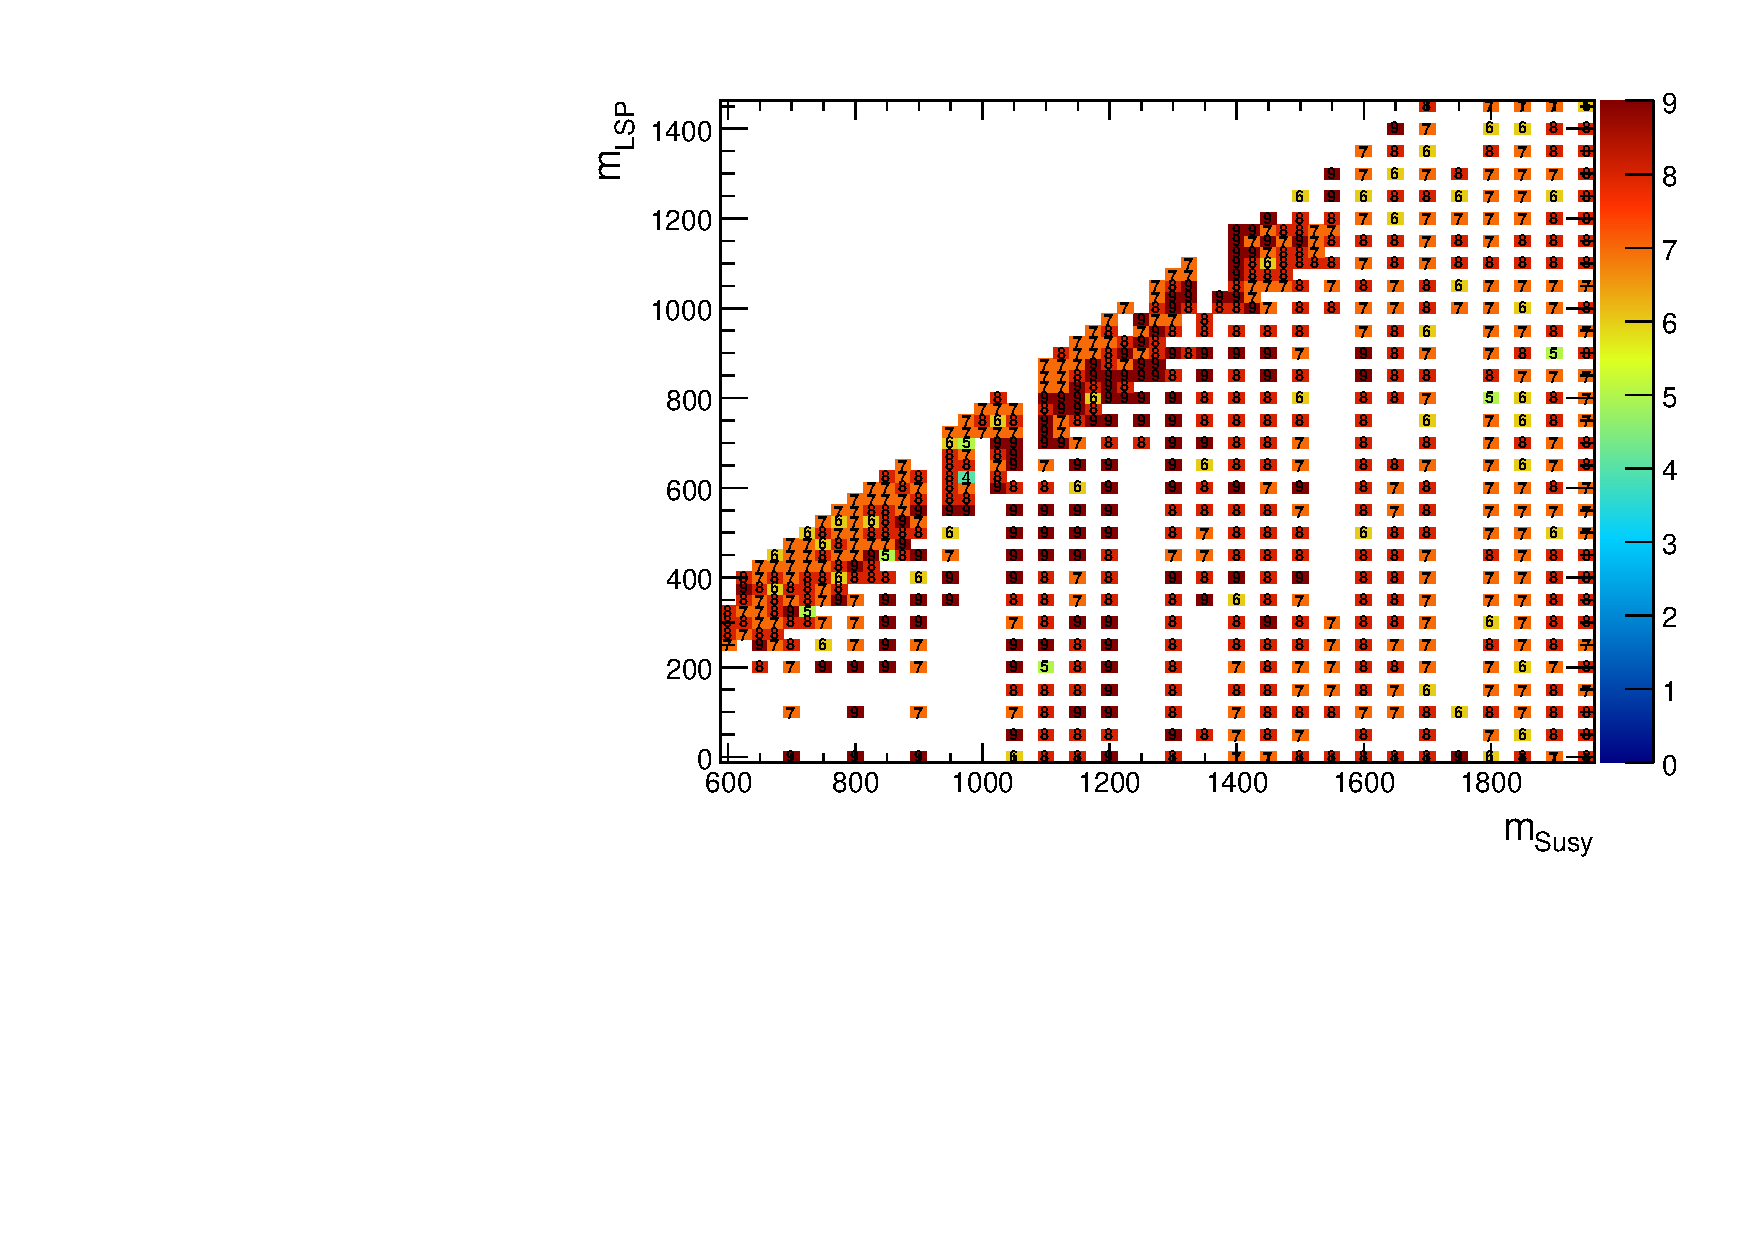
\includegraphics[width=0.33\textwidth]{figures/jetRanking/jetRankingT1tttt_order2/T1tttt_eq2a}} ~~
    \subfigure[eq1j]{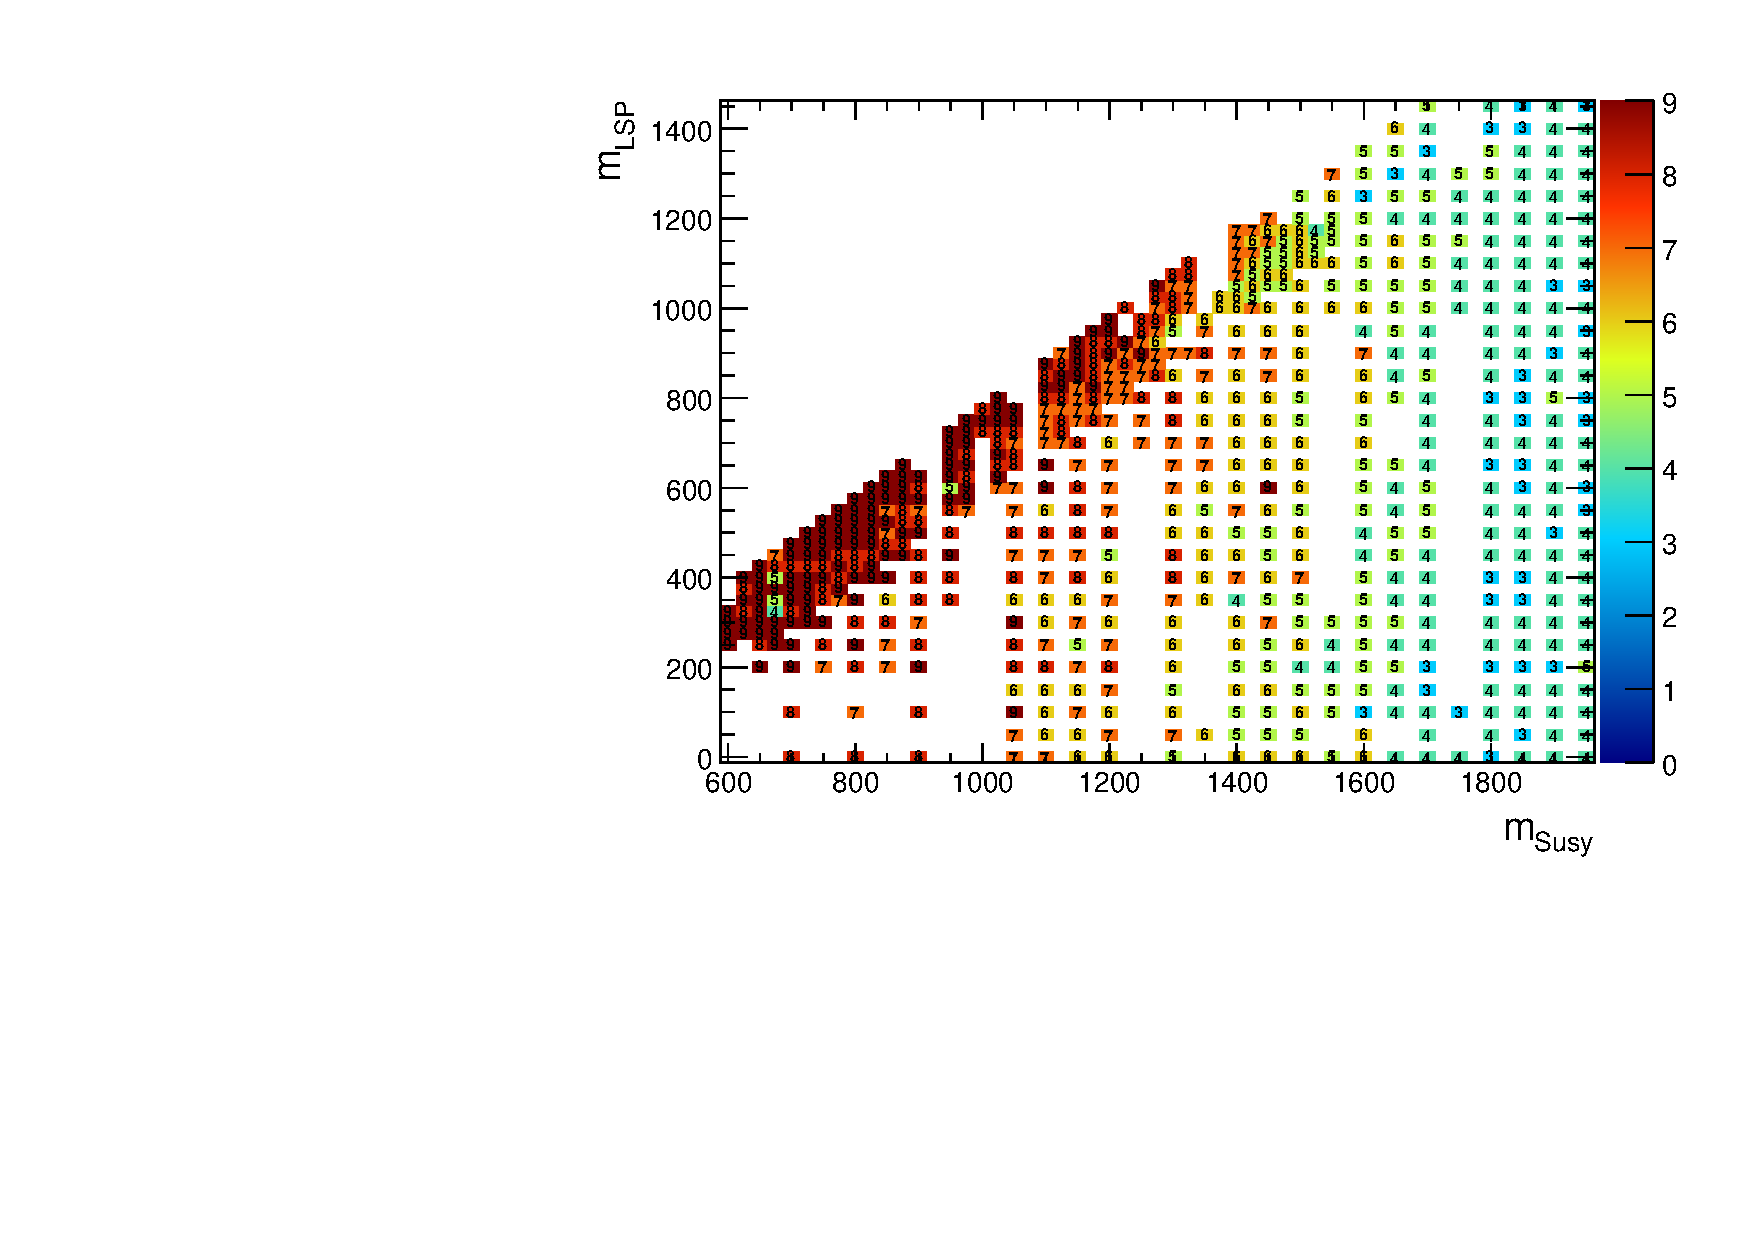
\includegraphics[width=0.33\textwidth]{figures/jetRanking/jetRankingT1tttt_order2/T1tttt_eq1j}} \\
  \end{center}
\end{figure}
